\begin{frame}
        \frametitle{DDCA Overview}
        \begin{itemize}
                  \setlength{\itemindent}{1cm}
                \item[\textbf{Title:}] Demand-Driven Cycamore Archetypes 
                \item[\textbf{PI:}] Anthony Scopatz, University of South 
                        Carolina\footnote{Anthony departed academia in year 2 
                        of the project. The PIship was transferred to Travis 
                        Knight at USC}
                \item[\textbf{Co-PI:}] Kathryn Huff, University of Illinois at 
                        Urbana-Champaign
                \item[\textbf{Start:}] October, 2016
                \item[\textbf{End:}] October, 2017
                \item[\textbf{Objectives:}] Develop an in situ demand 
                        driven development schedule calculation through 
                        non-optimizing, deterministic-optimizing, and 
                        stochastic-optimizing algorithms as Cyclus archetypes. 
                        Demonstrate these new archetypes in program-supporting 
                        fuel cycle scenarios.
        \end{itemize}
\end{frame}


\begin{frame}
        \frametitle{Quick Statistics}
        \begin{block}{Publications Affiliated with this Work}
                \begin{itemize}
                  \setlength{\itemindent}{3cm}
                        \item[\textbf{Journal Articles}] 3 (2 upcoming)
                        \item[\textbf{Full Conference Papers}] 3 (2 upcoming) 
                        \item[\textbf{Conference Summaries}] 7
                        \item[\textbf{Technical Reports}] 2 (1 upcoming)
                        \item[\textbf{Theses}] 1MS (2 upcoming)
                \end{itemize}
        \end{block}

                \begin{block}{Students Supported}
                        The funding supported graduate students and 
                        occasional undergraduates at UIUC.
                        \textbf{Jin Whan Bae} recieved his MS and is now at 
                        ORNL purusing Cyclus usability.
                        \textbf{Gwendolyn Chee} is writing an MS thesis related 
                        to this work and related work conducted at ANL with Bo Feng.
                        Undergraduate \textbf{Louis Kissinger} is a 
                        baccalaureate researcher this year in MCS at ANL.
                        Others include \textbf{Roberto Fairhurst}, \textbf{Gyu 
                        Tae Park}, \textbf{Snehal Chandan}, and \textbf{Aditya 
                        Bhosale}.
                \end{block}
\end{frame}

\begin{frame}
  \frametitle{Motivation}
  % a comment
        \begin{block}{Main Objective}
              To improve usability of Cyclus for transition scenarios.
        \end{block}
        

        \begin{block}{Main Challenge}
              Deploying reactors to meet power demand is trivial, and existed 
                in the earliest versions of Cyclus.
              \textbf{Automated, predictive deployment and decommissioning of 
                other facilities is more complex.} These include mining, 
                milling, enrichment, fuel 
                fabrication, reprocessing, and others. 

              For example, a balanced closed fuel cycle may require ensuring 
                that there is enough fast reactor fuel for their operation and 
                may drive deployment of a fleet of light water reactors.
        \end{block}
\end{frame}

\begin{frame}
\frametitle{Goals}
\textbf{Goals of this work} 
\begin{itemize}
	\item Develop demand driven deployment capabilities in \Cyclus (\deploy)
	\item Demonstrate the use of \deploy to set up EG01-23, EG01-24, EG01-29
	EG01-30 transition scenarios with constant and linearly increasing 
	power demand curves. 
\end{itemize}

\end{frame}

\begin{frame}
\frametitle{Method}
\begin{block}{Because Cyclus is Agent-Based}
	\begin{itemize}
		\item Its regions and institutions have the agency to dynamically make and alter deployment decisions.
		\item Each agent can make their own predictions of the future based on current and past performance of the simulation.
	\end{itemize}
	
	We embedded advanced time series prediction algorithms to automatically
	deploy fuel cycle facilities for the user. This was implemented
	in \textbf{\texttt{d3ploy}}, an Institution agent.
\end{block}
\end{frame}

%\begin{frame}
%  \frametitle{Goal of the Project}
%  % a comment
%  \begin{itemize}
%    \item[$\bullet$] Three types of methods were looked at for doing the prediction.
%    \item[$\bullet$] Non-optimizing methods. These methods included moving average
%                     , autoregressive moving average (ARMA), and autoregressive
%                     heteroskidasticity (ARCH) models.
%    \item[$\bullet$] Deterministic models. These models use a methodology that will
%                     always return the same answer given a unique input. This includes
%                     Fast Fourier Transforms, Exponential Smoothing, Holt-Winters,
%                     Polynomial regression.
%    \item[$\bullet$] Stochastic models. With stochastic models, the output is based
%                     on randomly sampling models to determine the behavior of the
%                     next time step. The method implimented here is a machine learning
%                     seasonal method.
%   \end{itemize}
%\end{frame}
%

\begin{frame}
\frametitle{Motivation}

\textbf{Gap in capability: User must define when support facilities are deployed}

\begin{figure}[htbp!]
\begin{center}
	
\includegraphics[width=0.8\textwidth]{images/user-deploy}
\end{center}
\caption{User defined Deployment Scheme }
\end{figure}

\textbf{Bridging the gap: Developed demand-driven deployment capability in \Cyclus. This capability is named \deploy.}

\begin{figure}[htbp!]
\begin{center}
	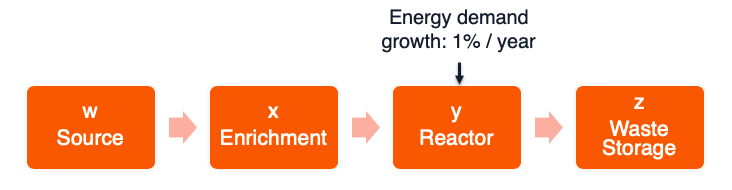
\includegraphics[width=0.8\textwidth]{images/auto-deploy}
\end{center}
\caption{Demand Driven Deployment Scheme}
\end{figure}

\end{frame}

\begin{frame}
\frametitle{Synergistic Spent Nuclear Fuel Dynamics Within the European 
	Union}
\begin{itemize}
	\item Collaborative spent fuel management is materially feasible among nuclear
	nations in the  European Union.
	\item Collaborative EU spent fuel management could expedite a fast reactor
	technology transition in France.
	\item By using spent fuel from other EU nations, France can avoid
	building new light water reactors to support a transition to
	fast reactors.
\end{itemize}
\end{frame}


\begin{frame}
\frametitle{Deployment Timeline for French Transition}
110 SFRs (66 GWe) are deployed by 2076.
\begin{figure}[htbp!]
\begin{minipage}[b]{.45\linewidth}
	\begin{center}
		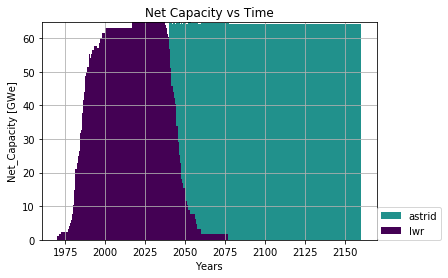
\includegraphics[width=\textwidth]{./images/french-transition/power_plot.png}
	\end{center}
	\caption{French Transition into an SFR Fleet}
	\label{fig:sfr_num}
\end{minipage}
\hspace{.5cm}
\begin{minipage}[b]{.45\linewidth}
	\centering
	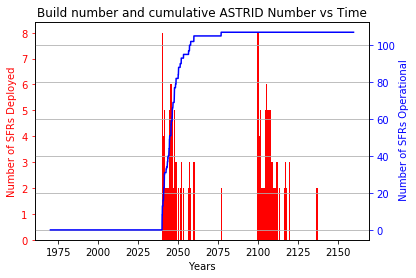
\includegraphics[width=\textwidth]{./images/french-transition/sfr_deploy.png}
	\caption{Deployment of French SFRs and total installed capacity}
	\label{fig:dep}
\end{minipage}
\end{figure}
\end{frame}



\begin{frame}
\begin{figure}[htbp!]
\begin{center}
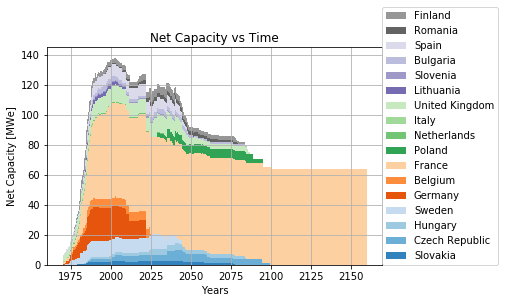
\includegraphics[width=\textwidth]{./images/onesim.png}
\end{center}
\caption{The simulated nuclear power deployment scheme relies on used
nuclear fuel collaboration among nations.
The historical operation of EU reactors is followed by the French transition to SFRs.  The steep transition from 2040 to 2060 reflects the scheduled decommissioning of reactors built in the 1975-2000 era of aggressive nuclear growth in France.}
\label{fig:tot_dep}
\end{figure}
\end{frame}

\begin{frame}
\frametitle{\deploy Objectives}
\textbf{\deploy's Main Objective}
\vspace{0.3em}
\\
Minimize the number of time steps of undersupply or under capacity 
of power.
\vspace{1em}
\\
\textbf{\deploy's Sub-Objectives}
\begin{itemize}
	\item Minimize the number of time steps of undersupply or under capacity 
	of any commodity.
	\item Minimize excessive oversupply of all commodities  
\end{itemize} 
\end{frame}

\begin{frame}
\frametitle{\deploy Input Parameters}
\begin{table}[]
\centering
\caption{\deploy's required and optional input parameters with examples.}
\label{tab:inputs}
\footnotesize
\begin{tabularx}{\textwidth}{l|LL}
	\hline
	& \textbf{Input Parameter}                                                           & \textbf{Examples}                                                                                                          \\ \hline
	\multirow{5}{*}{\textbf{Required}} & Demand driving commodity                                                           & Power, Fuel, Plutonium, etc.                                                                                                                      \\ 
	& Demand equation                                                                    & P(t) = 10000, sin(t), 10000*t                                                                                                                 \\ \cline{2-3} 
	& Facilities it controls                                                             & Fuel Fab, LWR reactor, SFR reactor, Waste repository, etc.                                                                                                      \\ \cline{2-3} 
	& Capacities of the facilities                                                       & 3000 kg, 1000 MW, 50000 kg                                                                                                     \\ \cline{2-3} 
	& Prediction method                                                                  & \begin{tabular}[c]{@{}l@{}}Power: fast fourier transform\\ Fuel: moving average\\ Spent fuel: moving average\end{tabular} \\ \cline{2-3} 
	& Deployment driven by & Installed Capacity/Supply                                                                                                                    \\ \hline
	\multirow{4}{*}{\textbf{Optional}} & Supply/Capacity Buffer type                                                                        & Absolute                                                                                                                  \\ \cline{2-3} 
	& Supply/Capacity Buffer size                                                                        & \begin{tabular}[c]{@{}l@{}}Power: 3000 MW\\ Fuel: 0 kg \\ Spent fuel: 0 kg\end{tabular}                                   \\ \cline{2-3} 
	& Facility preferences                                                               & \begin{tabular}[c]{@{}l@{}}LWR reactor = 100-t\\ SFR reactor = t-100 \end{tabular}          \\ \cline{2-3} 
	& Facility constraint                                                              & SFR reactor constraint = 5000kg of Pu            \\ \hline	
\end{tabularx}
\end{table}
\end{frame}

\begin{frame}
\frametitle{\deploy logic flow}
\begin{columns}
\column[t]{8cm}
\begin{figure}[]
\centering
\resizebox{0.7\textwidth} {0.45\height}{
	\begin{tikzpicture}[node distance=2cm]
	\tikzstyle{every node}=[font=\large]
	\node (Start) [bblock] {\textbf{Start of timestep ($t$).}};
	\node (Predict) [bblock, below of=Start] {\textbf{Calculate \\ $D_p(t+1)$ and $S_p(t+1)$ for a commodity}};
	\node (IsThere) [oblock, below of=Predict]{\textbf{$U(t+1) = S_p(t+1)-D_p(t+1)$}};
	\node (Deploy) [bblock, below of=IsThere, xshift = -3.5cm]{\textbf{Deployment of facility}};
	\node (NoDeploy) [bblock, right of=Deploy, xshift = 3.5cm]{\textbf{No Deployment} };
	\node (All) [oblock, below of=Deploy, xshift = 3.5cm] {\textbf{Is this done for all commodities?}};
	\node (End) [bblock, below of=All] {\textbf{Proceed to next timestep.}};
	
	\draw [arrow] (Start) -- (Predict); 
	\draw [arrow] (Predict) -- (IsThere);
	\draw [arrow] (IsThere) -- node[anchor=east] {$U(t+1) <$ buffer} (Deploy);
	\draw [arrow] (IsThere) -- node[anchor=west] {$U(t+1) \geq$ buffer} (NoDeploy);
	\draw [arrow] (Deploy) -- (All);
	\draw [arrow] (NoDeploy) -- (All);
	\draw [arrow] (All) -- node[anchor=west] {yes} (End);
	\draw [arrow] (All) -- ([shift={(-3.9cm,0.7cm)}]All.south west)-- node[anchor=east] {no} ([shift={(-3.9cm,-0.7cm)}]Predict.north west)--(Predict);
	\draw [arrow] (End) |-([shift={(3cm,-0.5cm)}]End.south east)-- ([shift={(3cm,0.5cm)}]Start.north east)-|(Start);
	\end{tikzpicture}
}
\caption{\deploy logic flow at every timestep in \Cyclus \cite{chee_demonstration_2019}.}
\label{fig:flow}
\end{figure}
\column[t]{5cm}
\vspace{2cm}
\\
$D_p : Predicted Demand$ \\
$S_p : Predicted Supply$ \\
$U = S_p-D_p$
\end{columns}
\end{frame}

\begin{frame}
\frametitle{\deploy Prediction Methods}
Non-Optimizing Methods 
\begin{itemize}
\item Moving Average (\texttt{ma})
\item Autoregressive Moving Average (\texttt{arma})
\item Autoregressive Heteroskedasticity (\texttt{arch})
\end{itemize}
Deterministic-Optimizing Methods 
\begin{itemize}
\item Fast Fourier Transform (\texttt{fft})
\item Polynomial Fit (\texttt{poly})
\item Exponential Smoothing
\item Triple Exponential Smoothing (\texttt{holt-winters})
\end{itemize}
Stochastic-Optimizing Methods 
\begin{itemize}
\item Auto-Regressive Integrated Moving Averages (\texttt{ARIMA})
\end{itemize}
\end{frame}

\begin{frame}
\frametitle{Breakdown of Results}
4 transition scenarios sought to minimize undersupply and under capacity of 
all commodities.
\begin{enumerate}
	\item EG01-23 ($P(t) = P_0$)
	\item EG01-24 ($P(t) = P_0 + rt$)
	\item EG01-29 ($P(t) = P_0)$
	\item EG01-30 ($P(t) = P_0 + rt$)
\end{enumerate}

This is achieved by:
\begin{enumerate}
	\item Comparison of prediction methods for each of 4 scenarios is conducted 
	to determine the best method. 
	\item Sensitivity analysis of power supply buffer is conducted to determine 
	best buffer size. 
	\item Using best prediction method, look ahead rate, buffer size, demonstrate \deploy 
	deploying reactor and supporting facilities to meet power demand 
	for 4 scenarios. 
\end{enumerate}

\end{frame}


\begin{frame}
\frametitle{EG01 - EG23}

\begin{figure}[H]
\centering
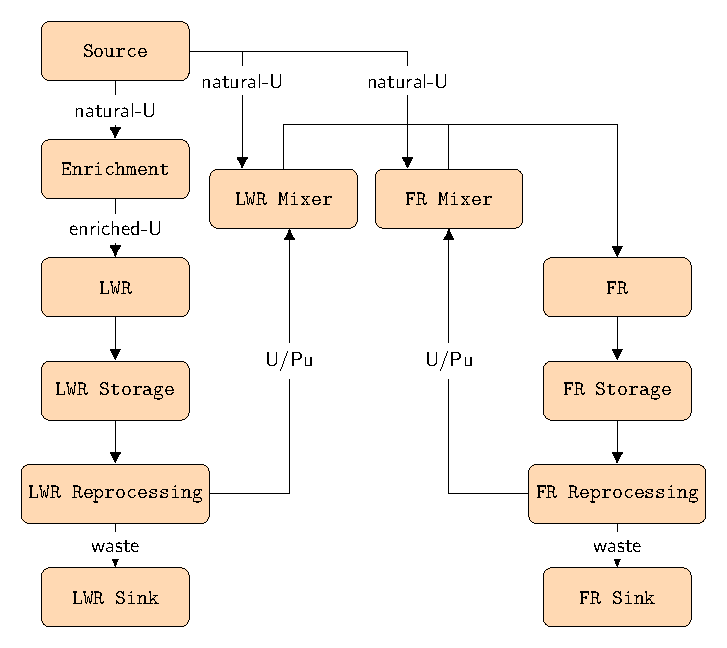
\includegraphics[width=0.6\textwidth]{images/23flow.pdf}
\hfill
\caption{EG01-EG23 fuel cycle as modeled in \Cyclus.}
\label{fig:23flow}
\end{figure}
\end{frame}

\begin{frame}
\frametitle{EG01 - EG30}

\begin{figure}[H]
\centering
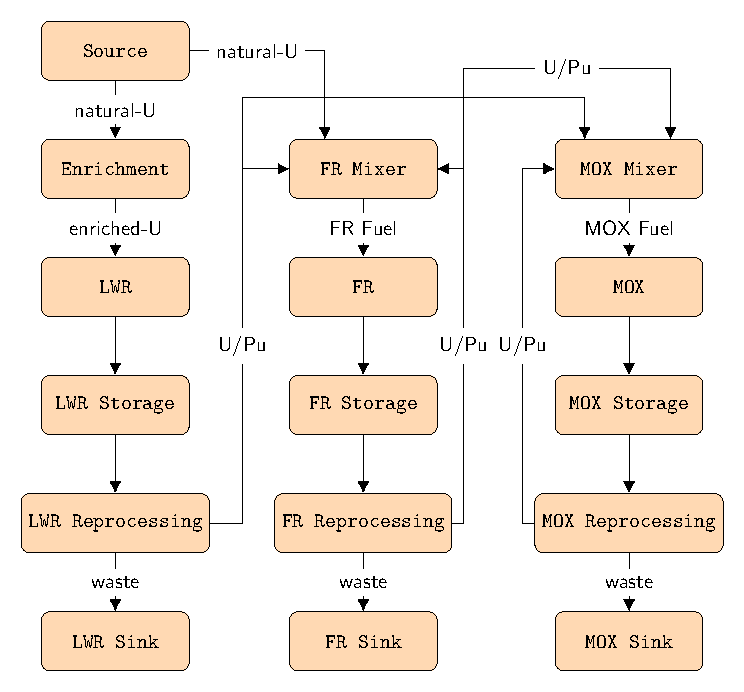
\includegraphics[width=0.7\textwidth]{images/29flow.pdf}
\hfill
\caption{EG01-EG30.}
\label{fig:30flow}
\end{figure}
\end{frame}

\begin{frame}
\frametitle{Comparison of Prediction Methods}
\textbf{EG01-23 Constant Power Demand Transition Scenario}

\begin{figure}[htbp!]
	\begin{center}
		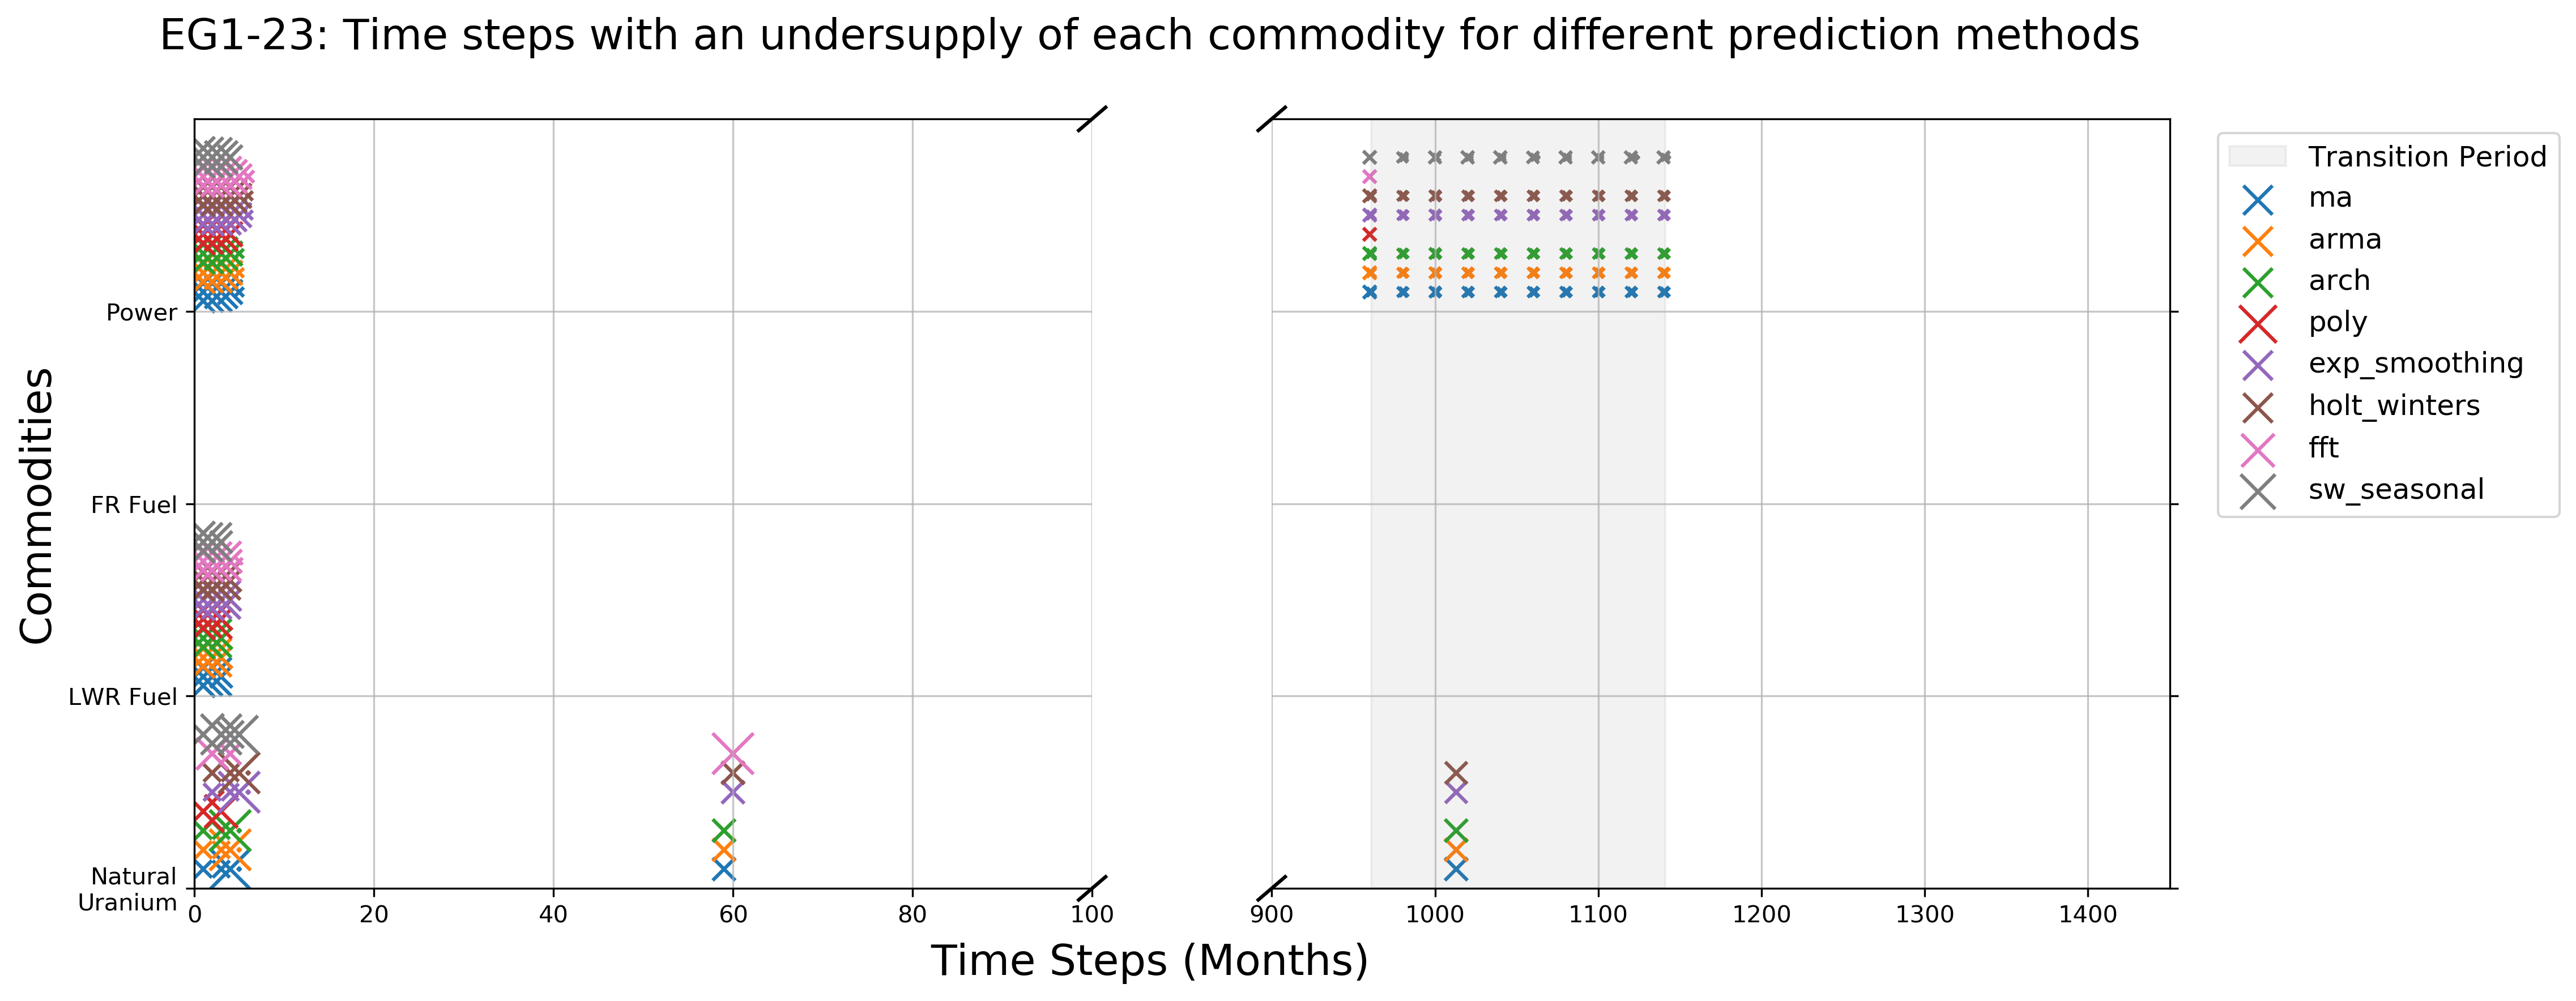
\includegraphics[width=\textwidth]{images/eg23-undersupply.png}
	\end{center}
	\caption{Time dependent undersupply of commodities for different
		prediction methods for the EG01-23 Transition Scenario with Constant Power Demand. The
		size of each cross is based on the size of the undersupply.
		Fewer crosses on plot indicates the method is more successful at preventing undersupply 
		of each commodity}
\end{figure}
\end{frame}

\begin{frame}
\frametitle{Comparison of Prediction Methods}
\textbf{EG01-23 Constant Power Demand Transition Scenario}
\begin{figure}[htbp!]
\begin{center}
	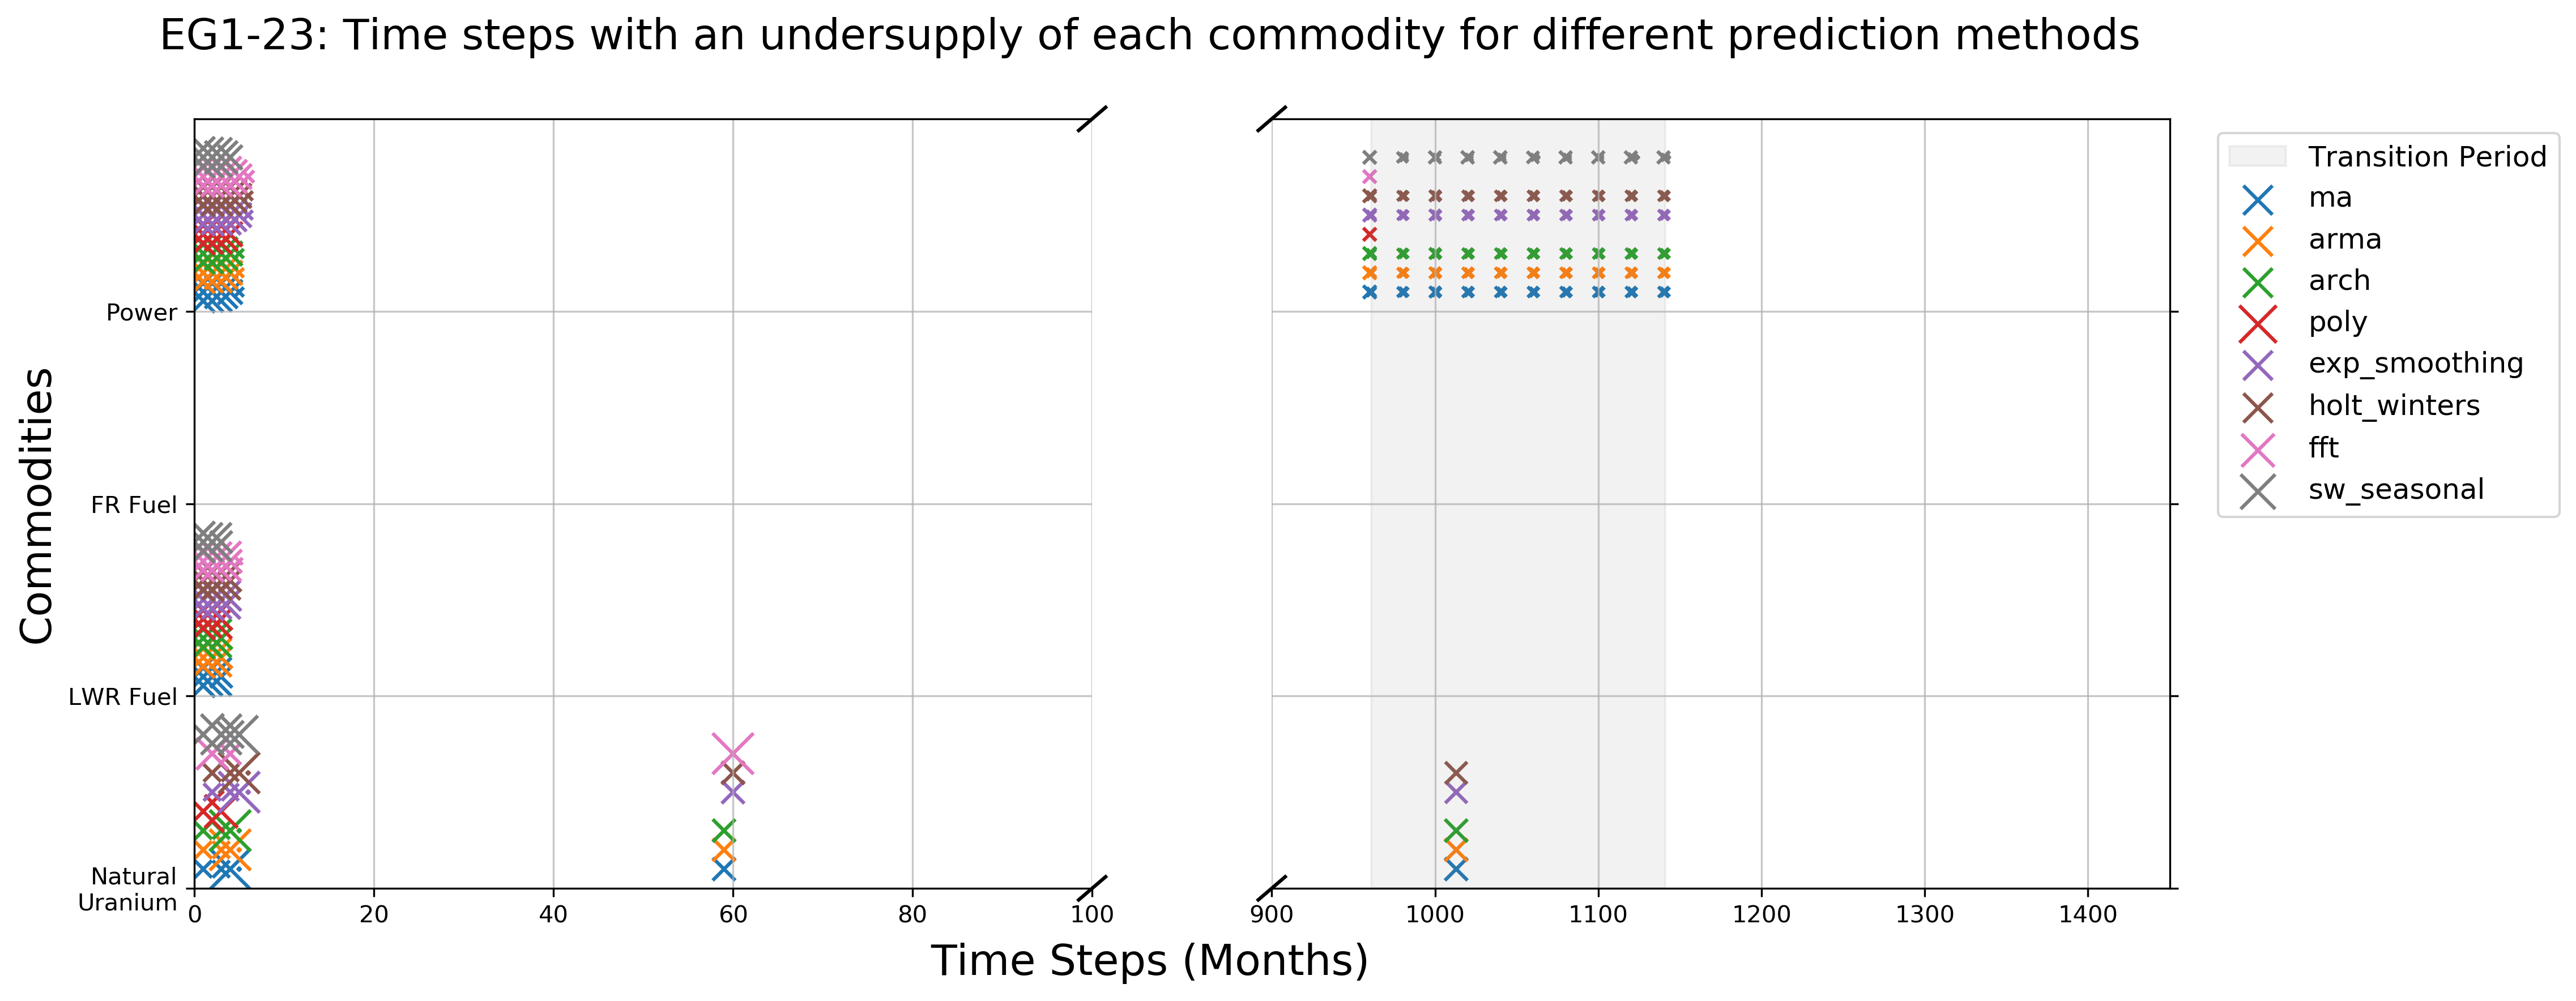
\includegraphics[width=\textwidth]{images/eg23-undersupply.png}
\end{center}
\caption{Time dependent undersupply of commodities for different
	prediction methods for the EG01-23 Transition Scenario with Constant Power Demand. The
	size of each cross is based on the size of the undersupply.
	Fewer crosses on plot indicates the method is more successful at preventing under capacity 
	of each commodity}
\end{figure}
\end{frame}

\begin{frame}
\frametitle{Comparison of Prediction Methods}
\textbf{EG01-24 Constant Power Demand Transition Scenario}
\begin{figure}[htbp!]
\begin{center}
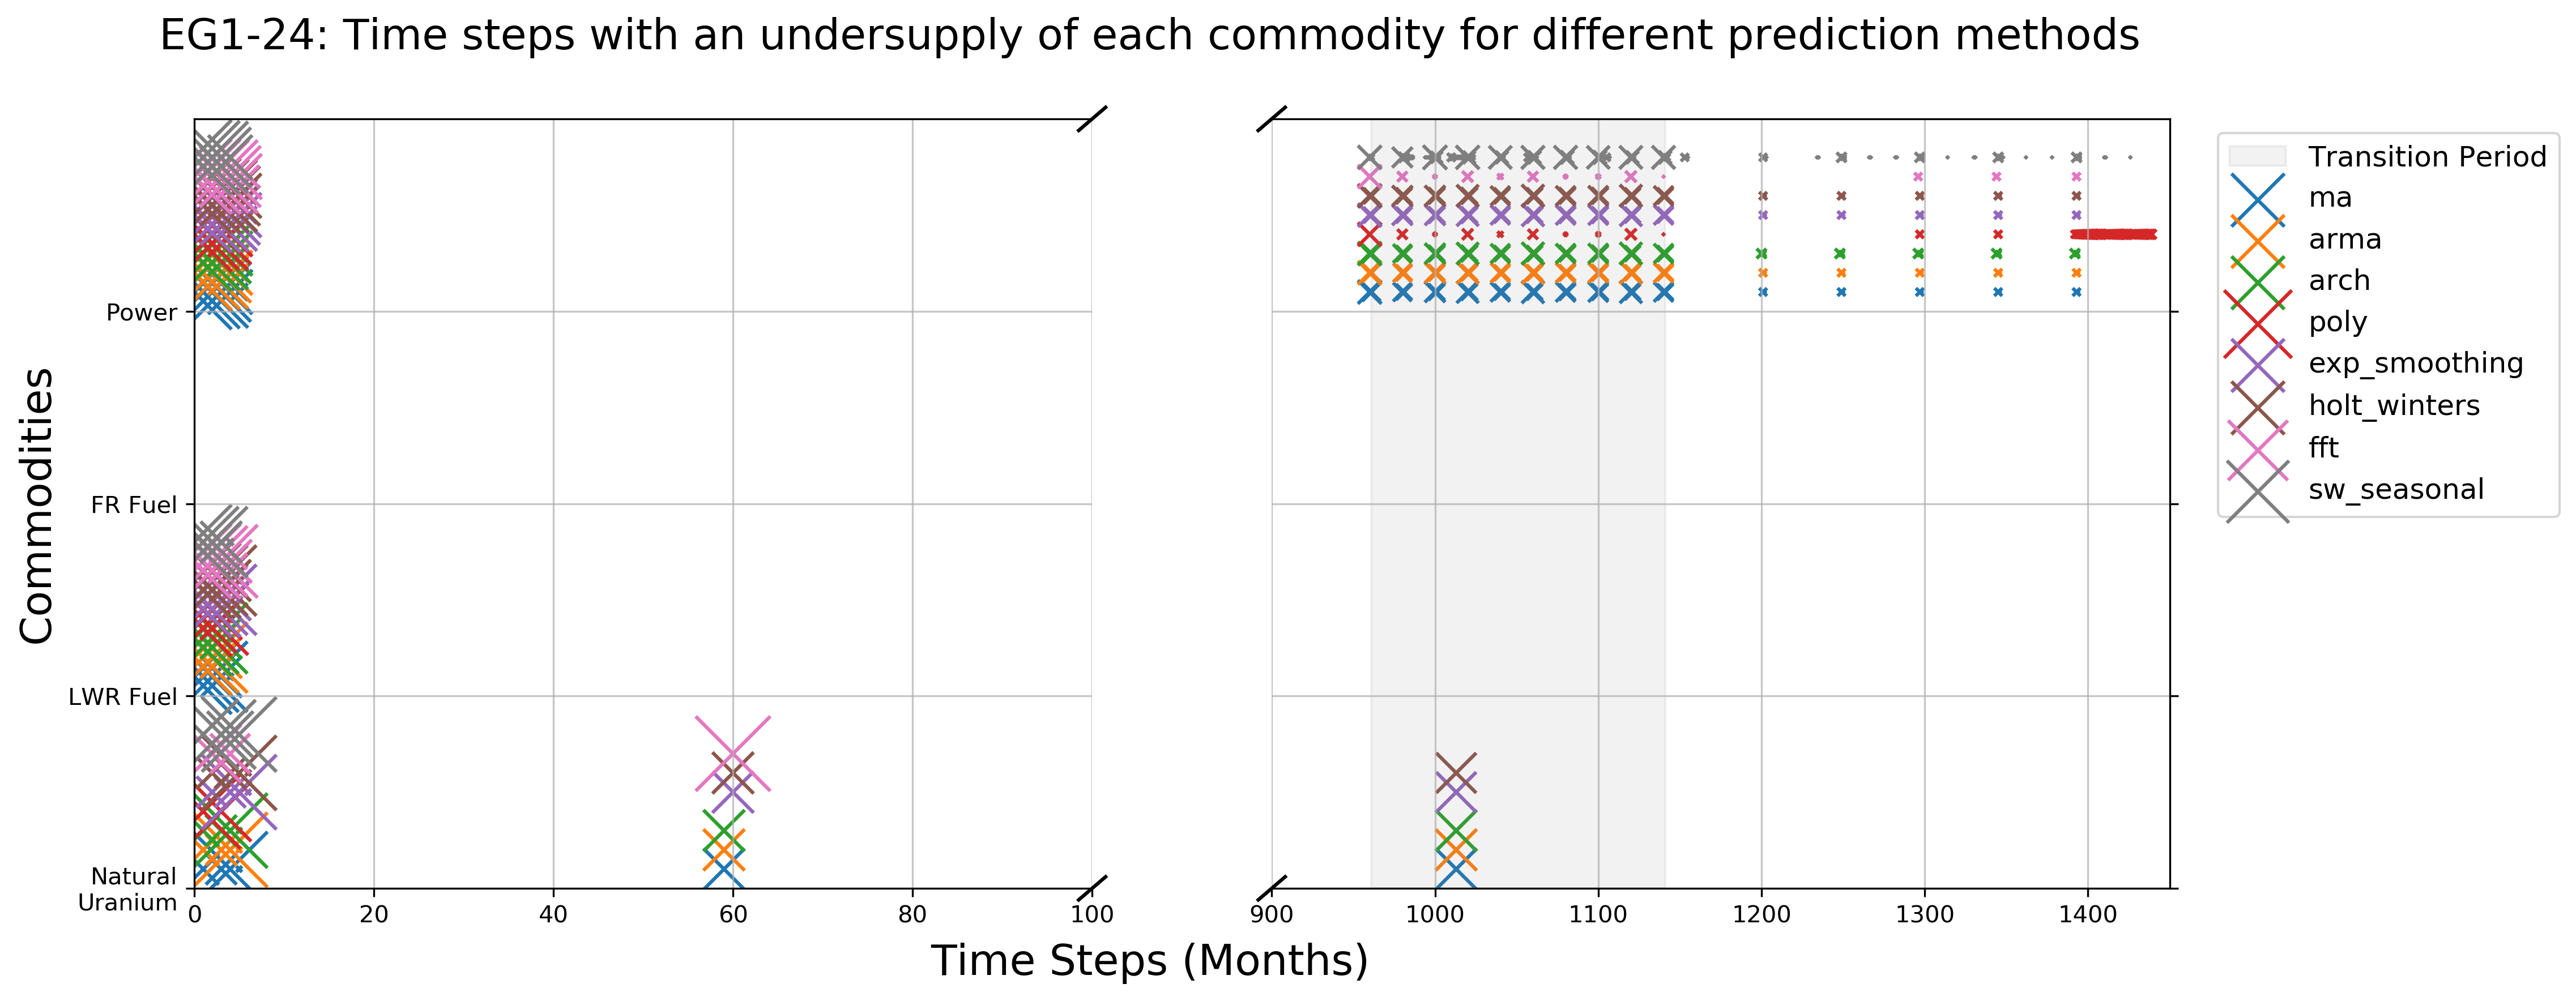
\includegraphics[width=\textwidth]{images/eg24-undersupply.png}
\end{center}
\caption{Time dependent undersupply of commodities for different
prediction methods for the EG01-24 Transition Scenario with Linearly Increasing Power Demand.The
size of each cross is based on the size of the undersupply.
Fewer crosses on plot indicates the method is more successful at preventing undersupply 
of each commodity}
\end{figure}
\end{frame}

\begin{frame}
\frametitle{Comparison of Prediction Methods}
\textbf{EG01-24 Constant Power Demand Transition Scenario}
\begin{figure}[htbp!]
\begin{center}
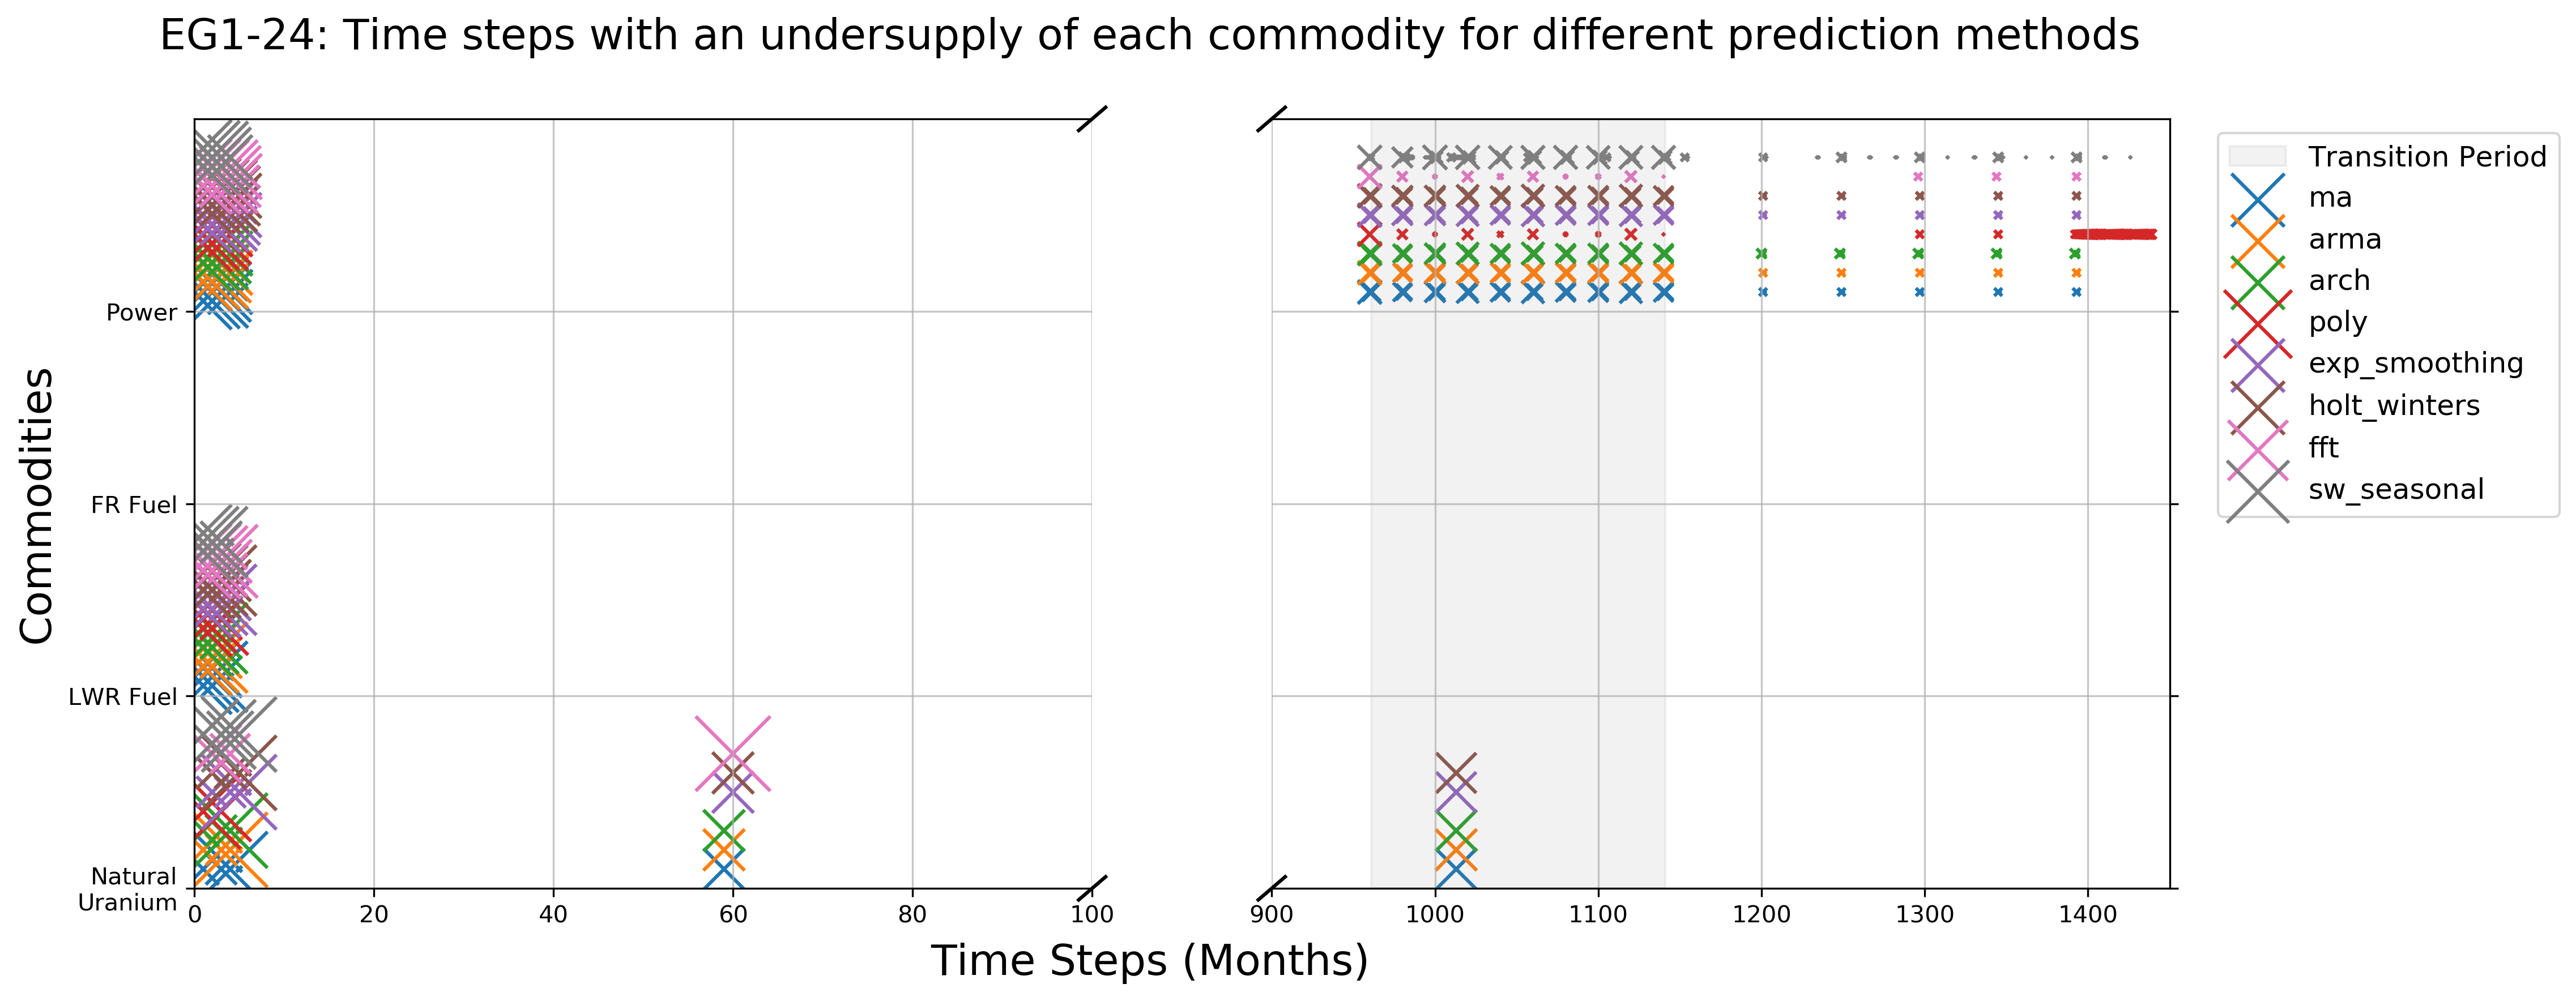
\includegraphics[width=\textwidth]{images/eg24-undersupply.png}
\end{center}
\caption{Time dependent undersupply of commodities for different
prediction methods for the EG01-24 Transition Scenario with Linearly Increasing Power Demand. The
size of each cross is based on the size of the under capacity.
Fewer crosses on plot indicates the method is more successful at preventing under capacity
of each commodity}
\end{figure}
\end{frame}

\begin{frame}
\frametitle{Comparison of Prediction Methods}
\textbf{Main Takeaway}
\\
The best performing prediction method for each transition scenario is: 
\begin{enumerate}
\item EG01-23 Constant Power Demand: \texttt{poly}
\item EG01-24 Linearly Increasing Power Demand: \texttt{fft}
\item EG01-29 Constant Power Demand: \texttt{poly}
\item EG01-30 Linearly Increasing Power Demand: \texttt{fft}
\end{enumerate}
\end{frame}

\begin{frame}
\frametitle{Sensitivity Analysis of Power Buffer}
\textbf{EG01-24}: Linearly Increasing Power Demand
\begin{figure}[htbp!]
	\begin{center}
		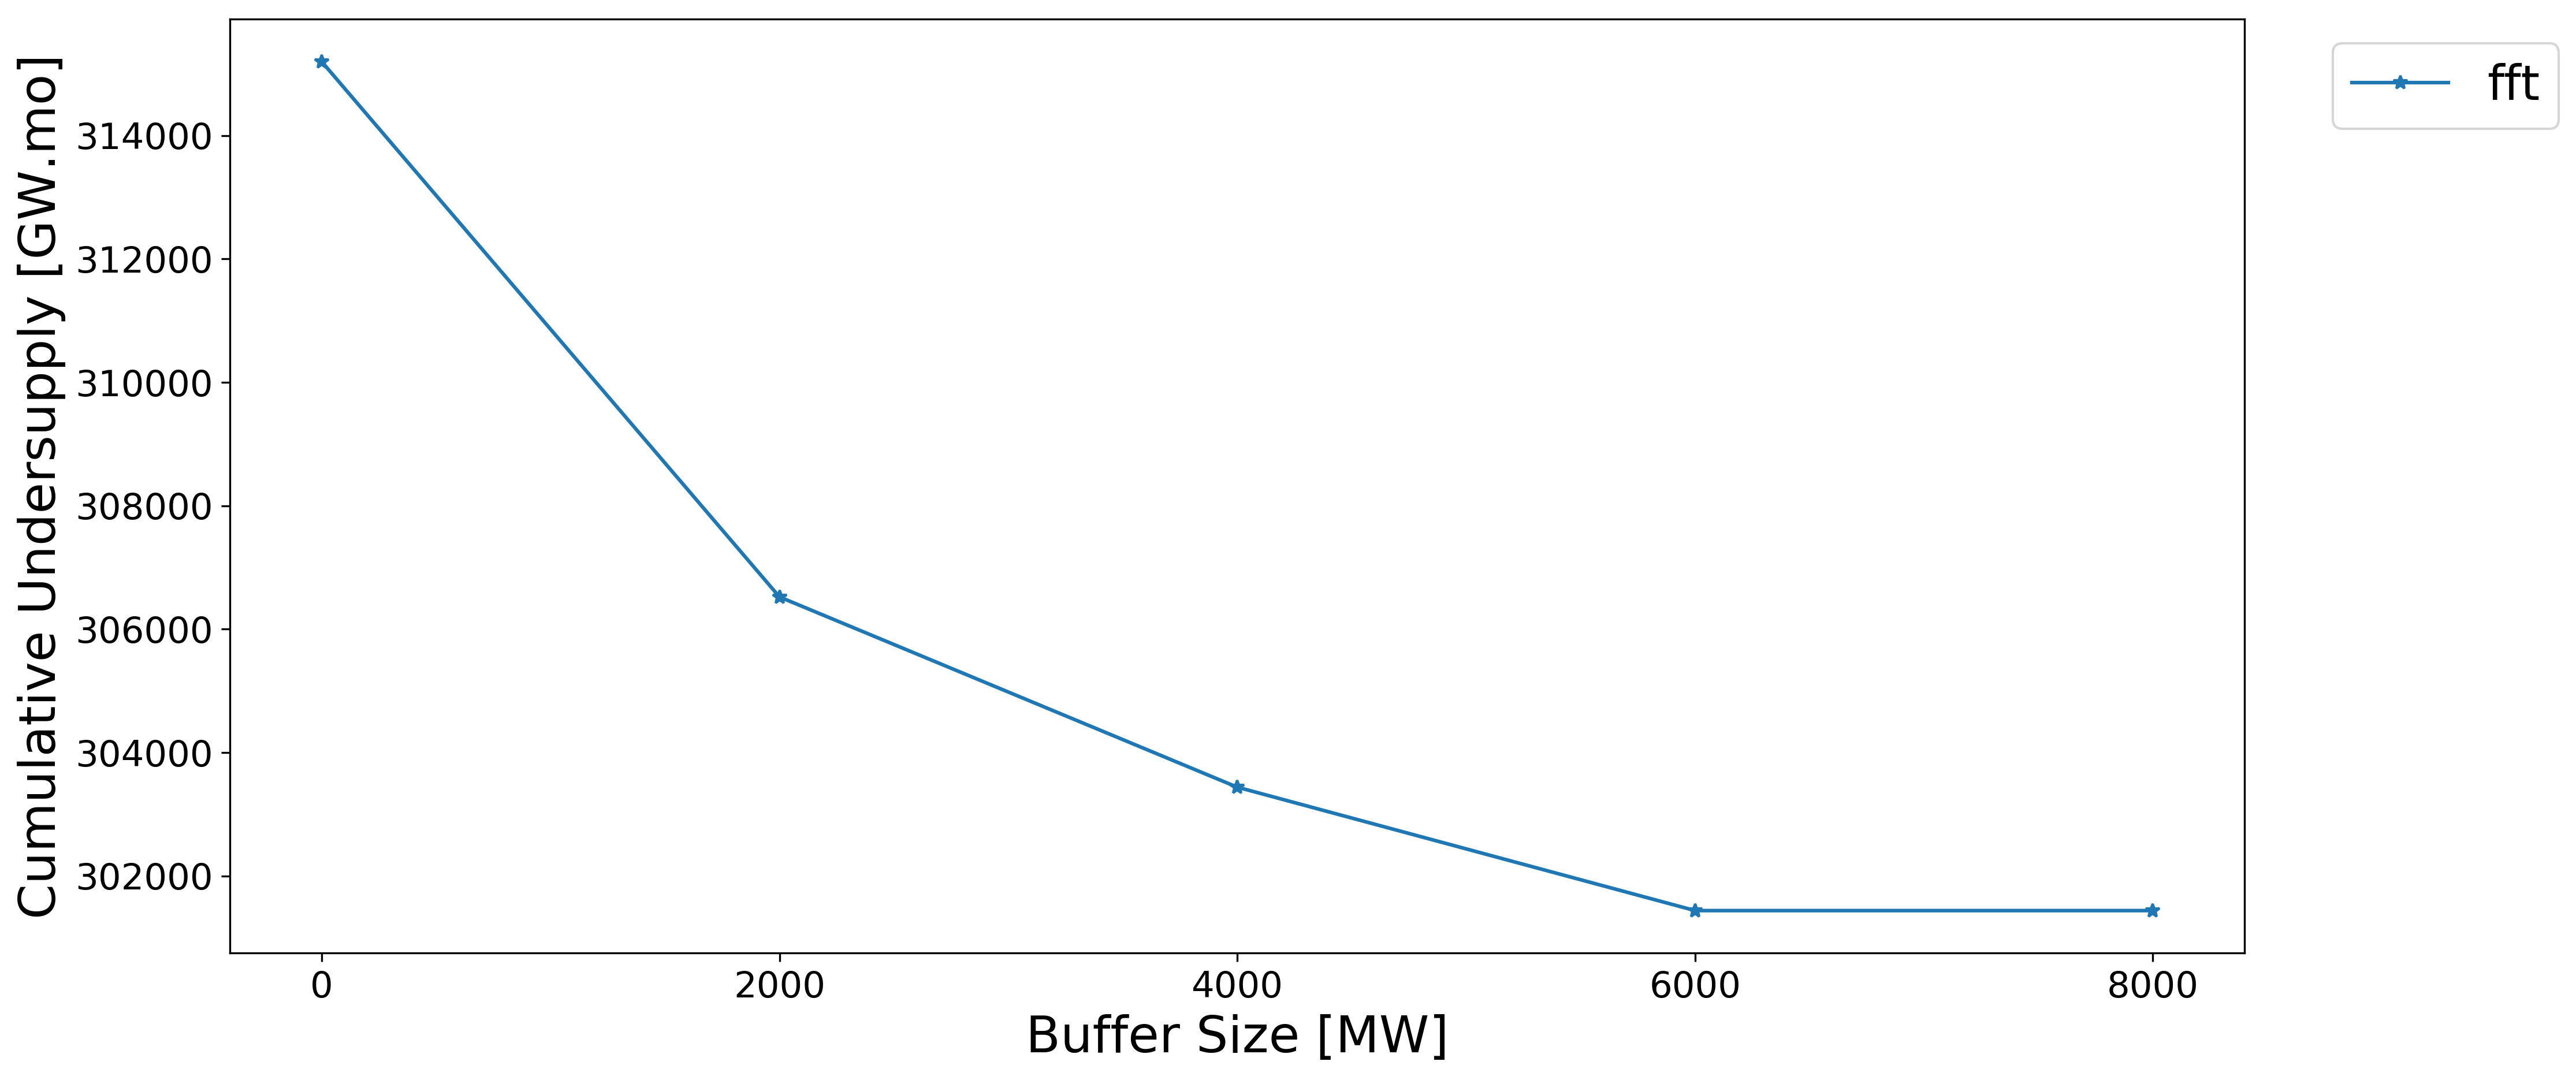
\includegraphics[width=0.8\textwidth]{images/24-sens-buffer}
	\end{center}
	\caption{Sensitivity Analysis of Power buffer size on cumulative 
		undersupply of Power for EG01-EG24 transition scenarios 
		with linearly increasing power demand using the fft prediction method.}
\end{figure}
\end{frame}

\begin{frame}
\frametitle{Sensitivity Analysis of Power Buffer}
\textbf{EG01-30}: Linearly Increasing Power Demand
\begin{figure}[htbp!]
\begin{center}
	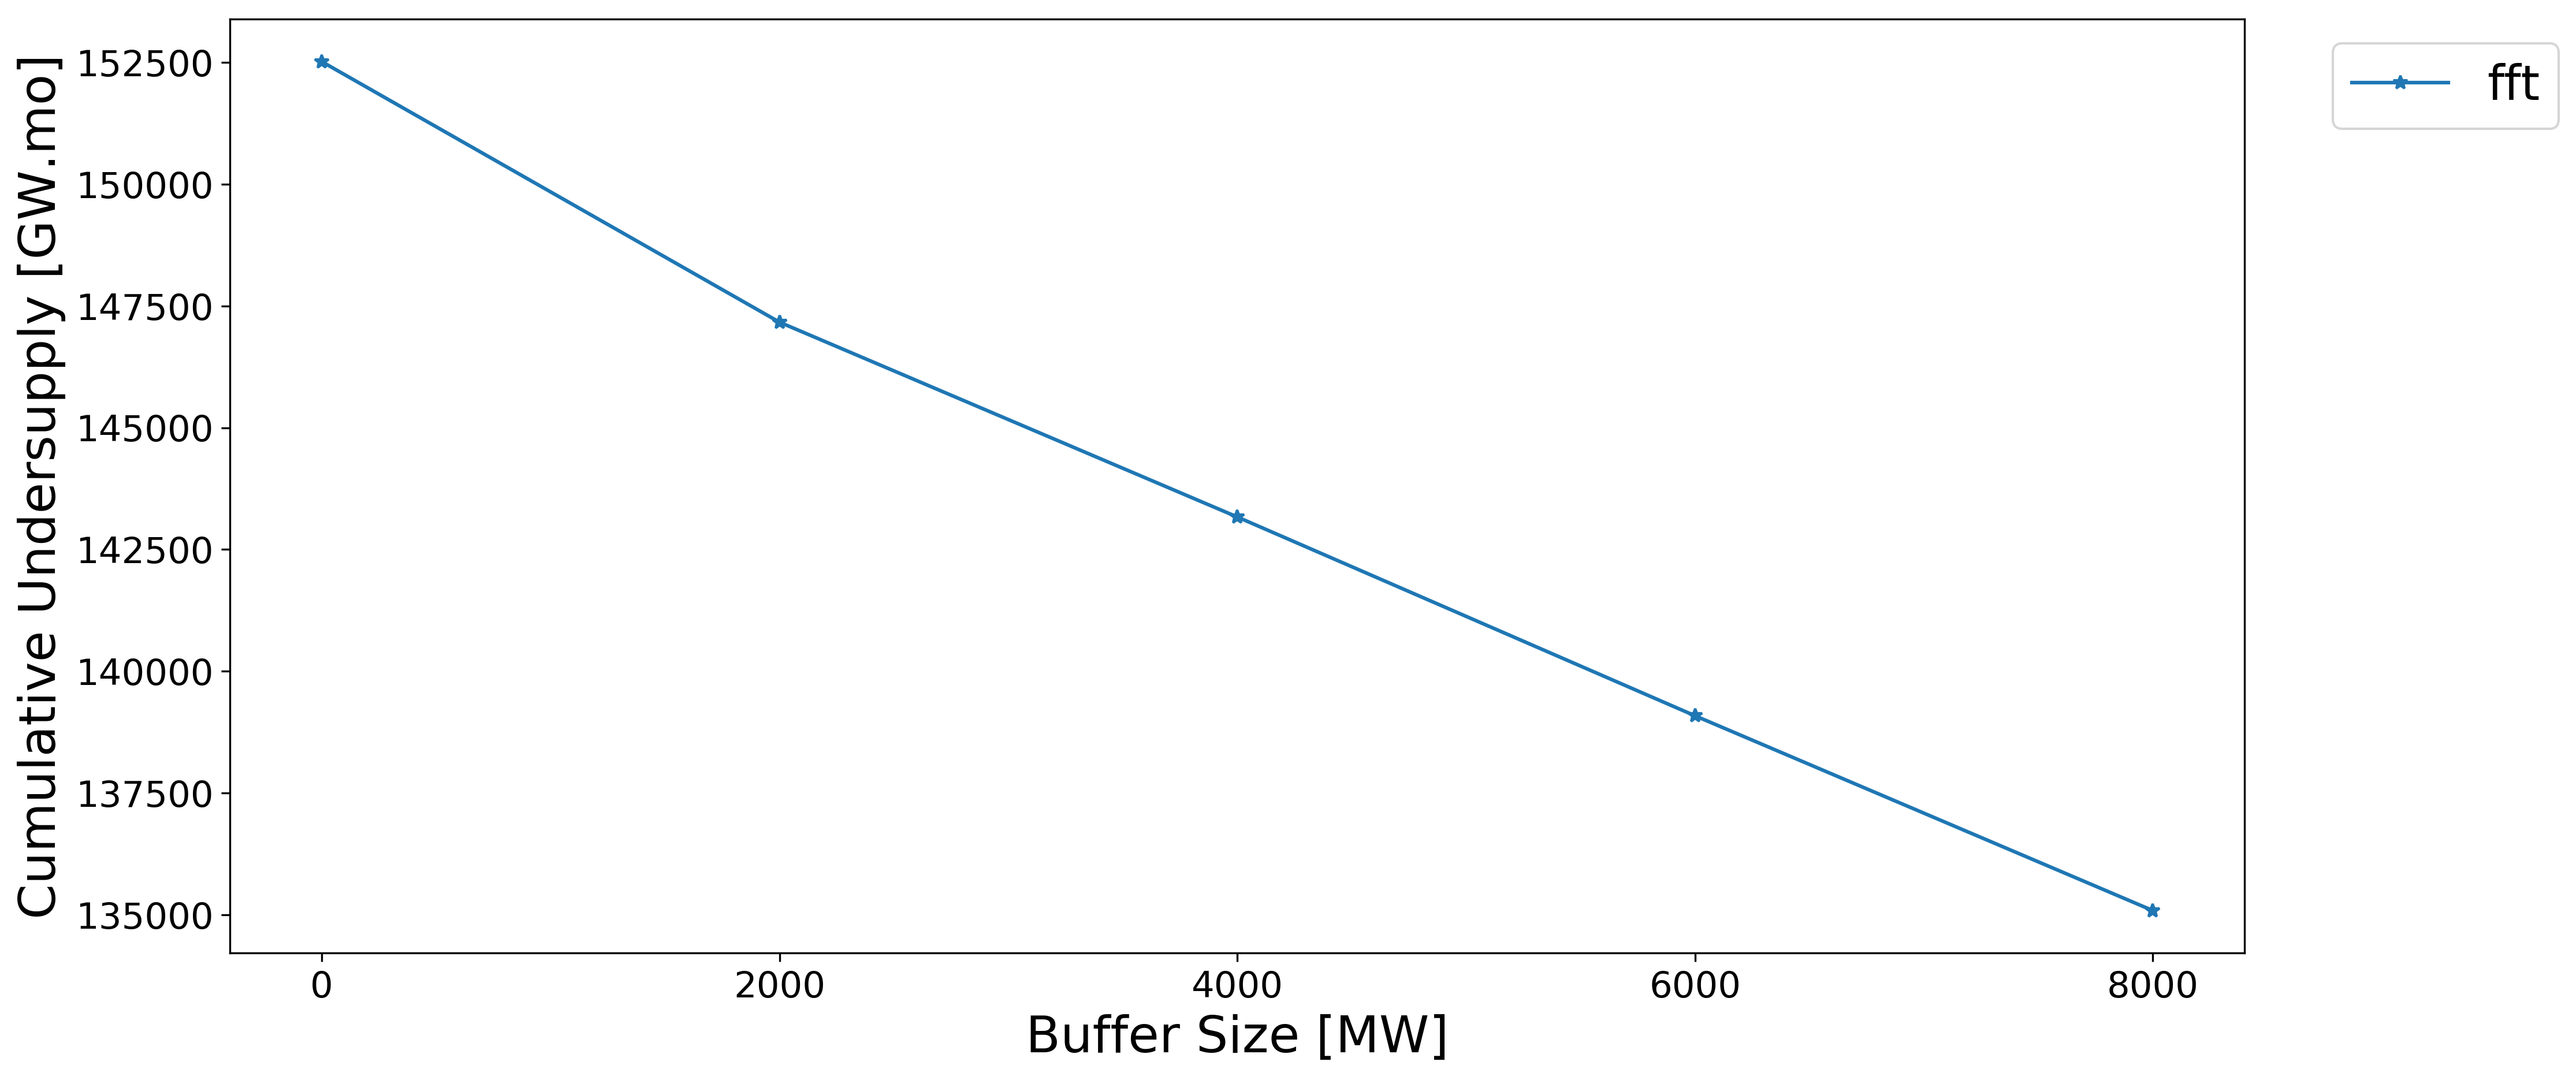
\includegraphics[width=0.8\textwidth]{images/30-sens-buffer}
\end{center}
\caption{Sensitivity Analysis of Power buffer size on cumulative 
	undersupply of Power for EG01-EG30 transition scenarios 
	with linearly increasing power demand using the fft prediction method.}
\end{figure}
\end{frame}

\begin{frame}
\frametitle{Sensitivity Analysis of Power Buffer}
\textbf{Main Takeaway}
\\
The best power supply buffer for each transition scenario is: 
\begin{enumerate}
\item EG01-23 Constant Power Demand: 0 MW
\item EG01-24 Linearly Increasing Power Demand: 6000 MW
\item EG01-29 Constant Power Demand: 0 MW
\item EG01-30 Linearly Increasing Power Demand: 8000 MW 
\end{enumerate}
\end{frame}

\begin{frame}
\frametitle{Best Performing Transition Scenarios}
\textbf{Input Parameters of best performing transition scenarios}
\begin{table}[]
	\resizebox{\textwidth}{!}{%
		\begin{tabular}{|l|l|c|l|l|l|}
			\hline
			\multirow{2}{*}{}                         & \multicolumn{1}{c|}{\multirow{2}{*}{\textbf{Input Parameter}}} & \multicolumn{4}{c|}{\textbf{Simulation Description}}                                                                                                                                                                                                                                                       \\ \cline{3-6} 
			& \multicolumn{1}{c|}{}                                          & \multicolumn{1}{l|}{\textbf{EG01-23}}                                                                 & \textbf{EG01-24}                  & \textbf{EG01-29}                 &\textbf{EG01-30}                                                  \\ \hline
			\multirow{4}{*}{\textbf{Required}} & Demand driving commodity                                       & \multicolumn{4}{c|}{Power}                                                                                                                                                                                                                                                                                 \\ \cline{2-6} 
			& Demand equation [MW]                                               & \multicolumn{1}{l|}{60000}                                                                                & $60000 + 250t/12$ & 60000                     &     $60000 + 250t/12$                                       \\ \cline{2-6} 
			& Prediction method                                              & \texttt{poly}       & \texttt{fft}             & \texttt{poly}         &  \texttt{fft}    \\ \cline{2-6} 
			& Deployment Driving Method                                      & \multicolumn{4}{c|}{Installed Capacity}                                                                                                                                                                                                                                                                    \\ \hline
			\multirow{2}{*}{\textbf{Optional}} & Buffer type                                                    & \multicolumn{4}{c|}{Absolute}                                                                                                                                                                                                                                                               \\ \cline{2-6} 
			& Power Buffer size [MW]                                                   & 0 & 6000 & 0 & 8000 \\ \hline
		\end{tabular}%
	}
	\caption{\deploy's input parameters for EG01-EG23, EG01-EG24, EG01-EG29, and 
		EG01-EG30 transition scenarios
		that minimizes undersupply of power and minimizes 
		the undersupply and under capacity of the other facilities. }
	\label{tab:bestinputs}
\end{table}
\end{frame}

\begin{frame}
\frametitle{Best Performing Transition Scenarios}
\textbf{EG01-23: Constant Power Demand}
\begin{figure}[htbp!]
\begin{center}
	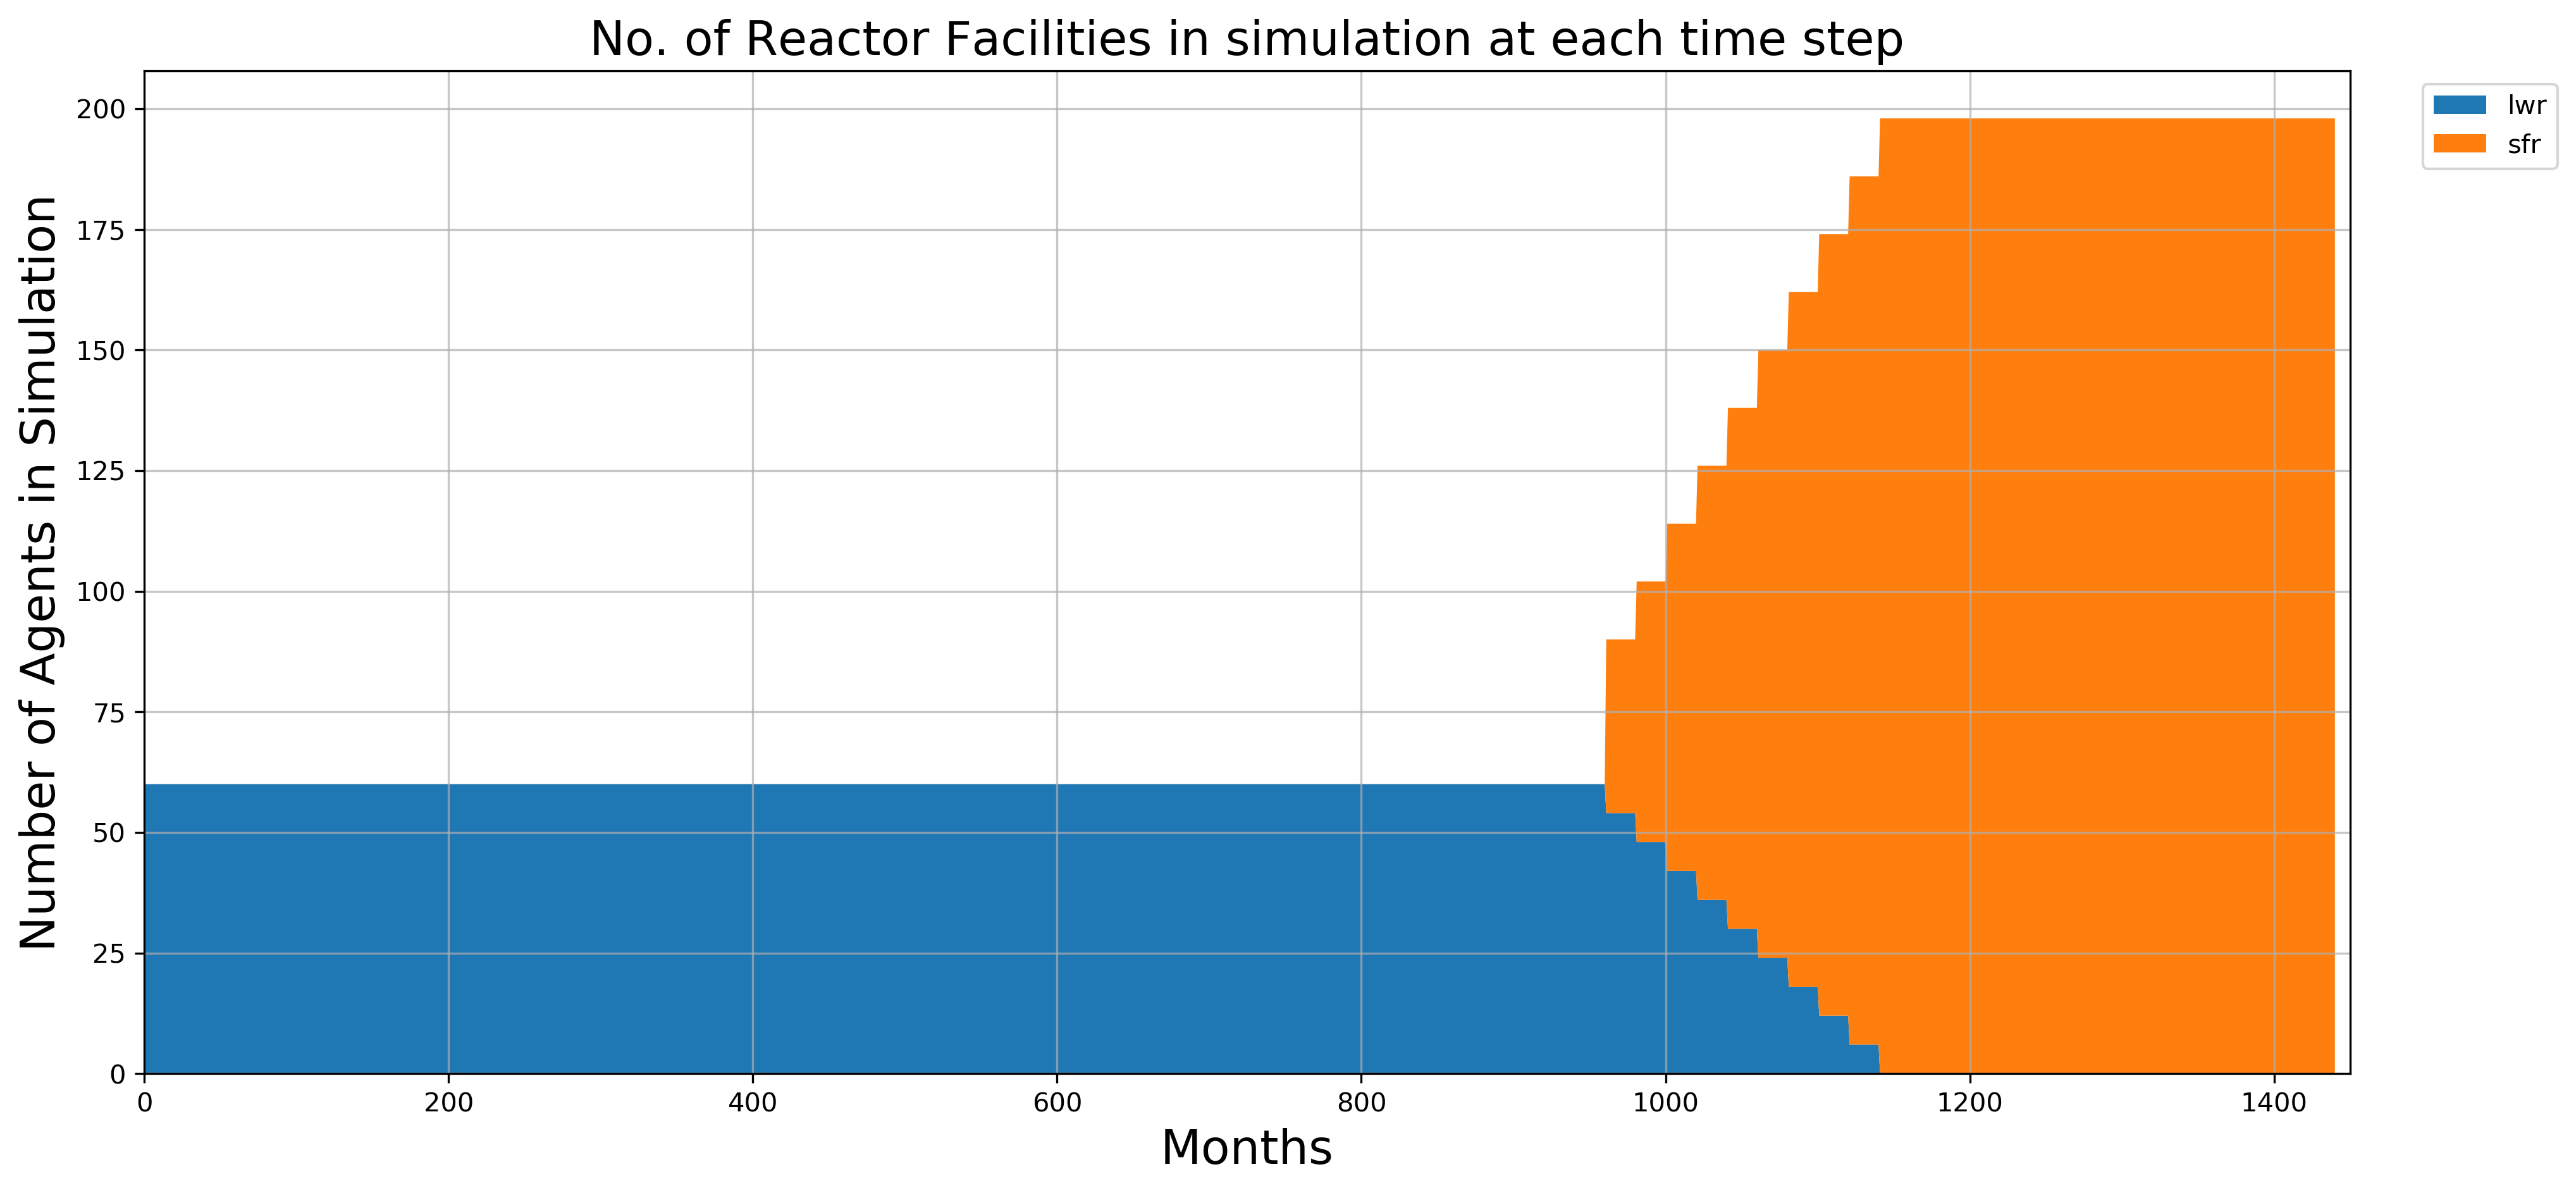
\includegraphics[width=\textwidth]{images/eg23-stack_reactor.png}
\end{center}
\caption{Time dependent deployment of reactor facilities in 
	the EG01-23 constant power demand transition scenario. 
	\deploy automatically deploys reactor facilities 
	to set up a supply chain to meet constant power demand of $60000$ MW
	during a transition from \glspl{LWR} to \glspl{SFR}}.
\end{figure}
\end{frame}

\begin{frame}
\frametitle{Best Performing Transition Scenarios}
\textbf{EG01-23: Constant Power Demand}
\begin{figure}[htbp!]
\begin{center}
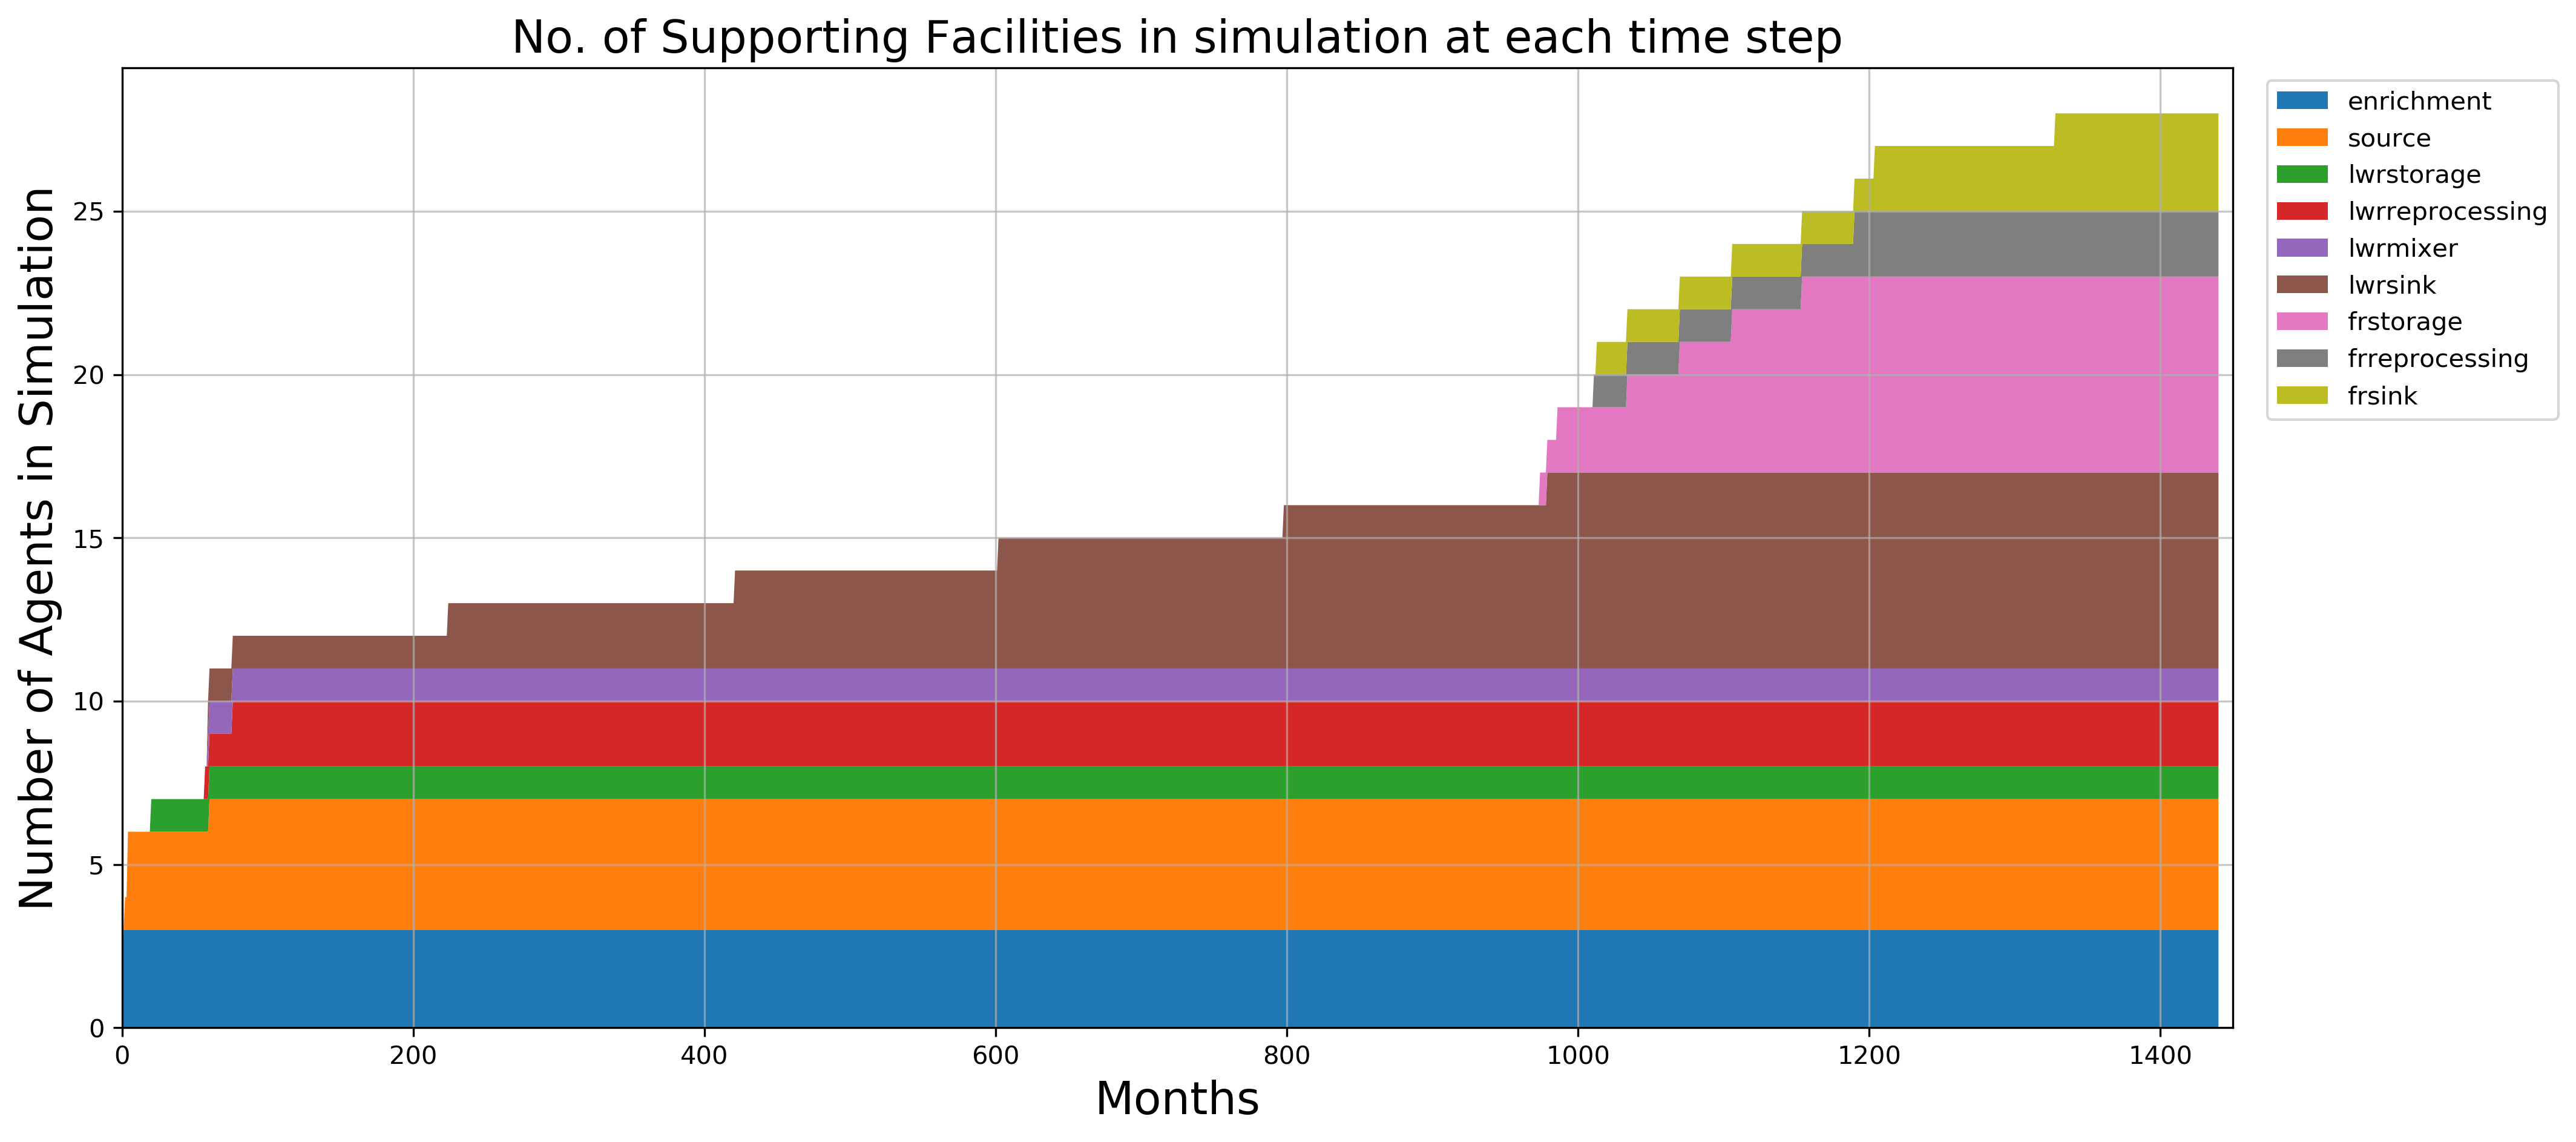
\includegraphics[width=\textwidth]{images/eg23-stack_support.png}
\end{center}
\caption{Time dependent deployment of supporting facilities in 
the EG01-23 constant power demand transition scenario. 
\deploy automatically deploys reactor facilities 
to set up a supply chain to meet constant power demand of $60000$ MW
during a transition from \glspl{LWR} to \glspl{SFR}}.
\end{figure}
\end{frame}

\begin{frame}
\frametitle{Best Performing Transition Scenarios}
\textbf{EG01-30: Linearly Increasing Power Demand}
\begin{figure}[htbp!]
\begin{center}
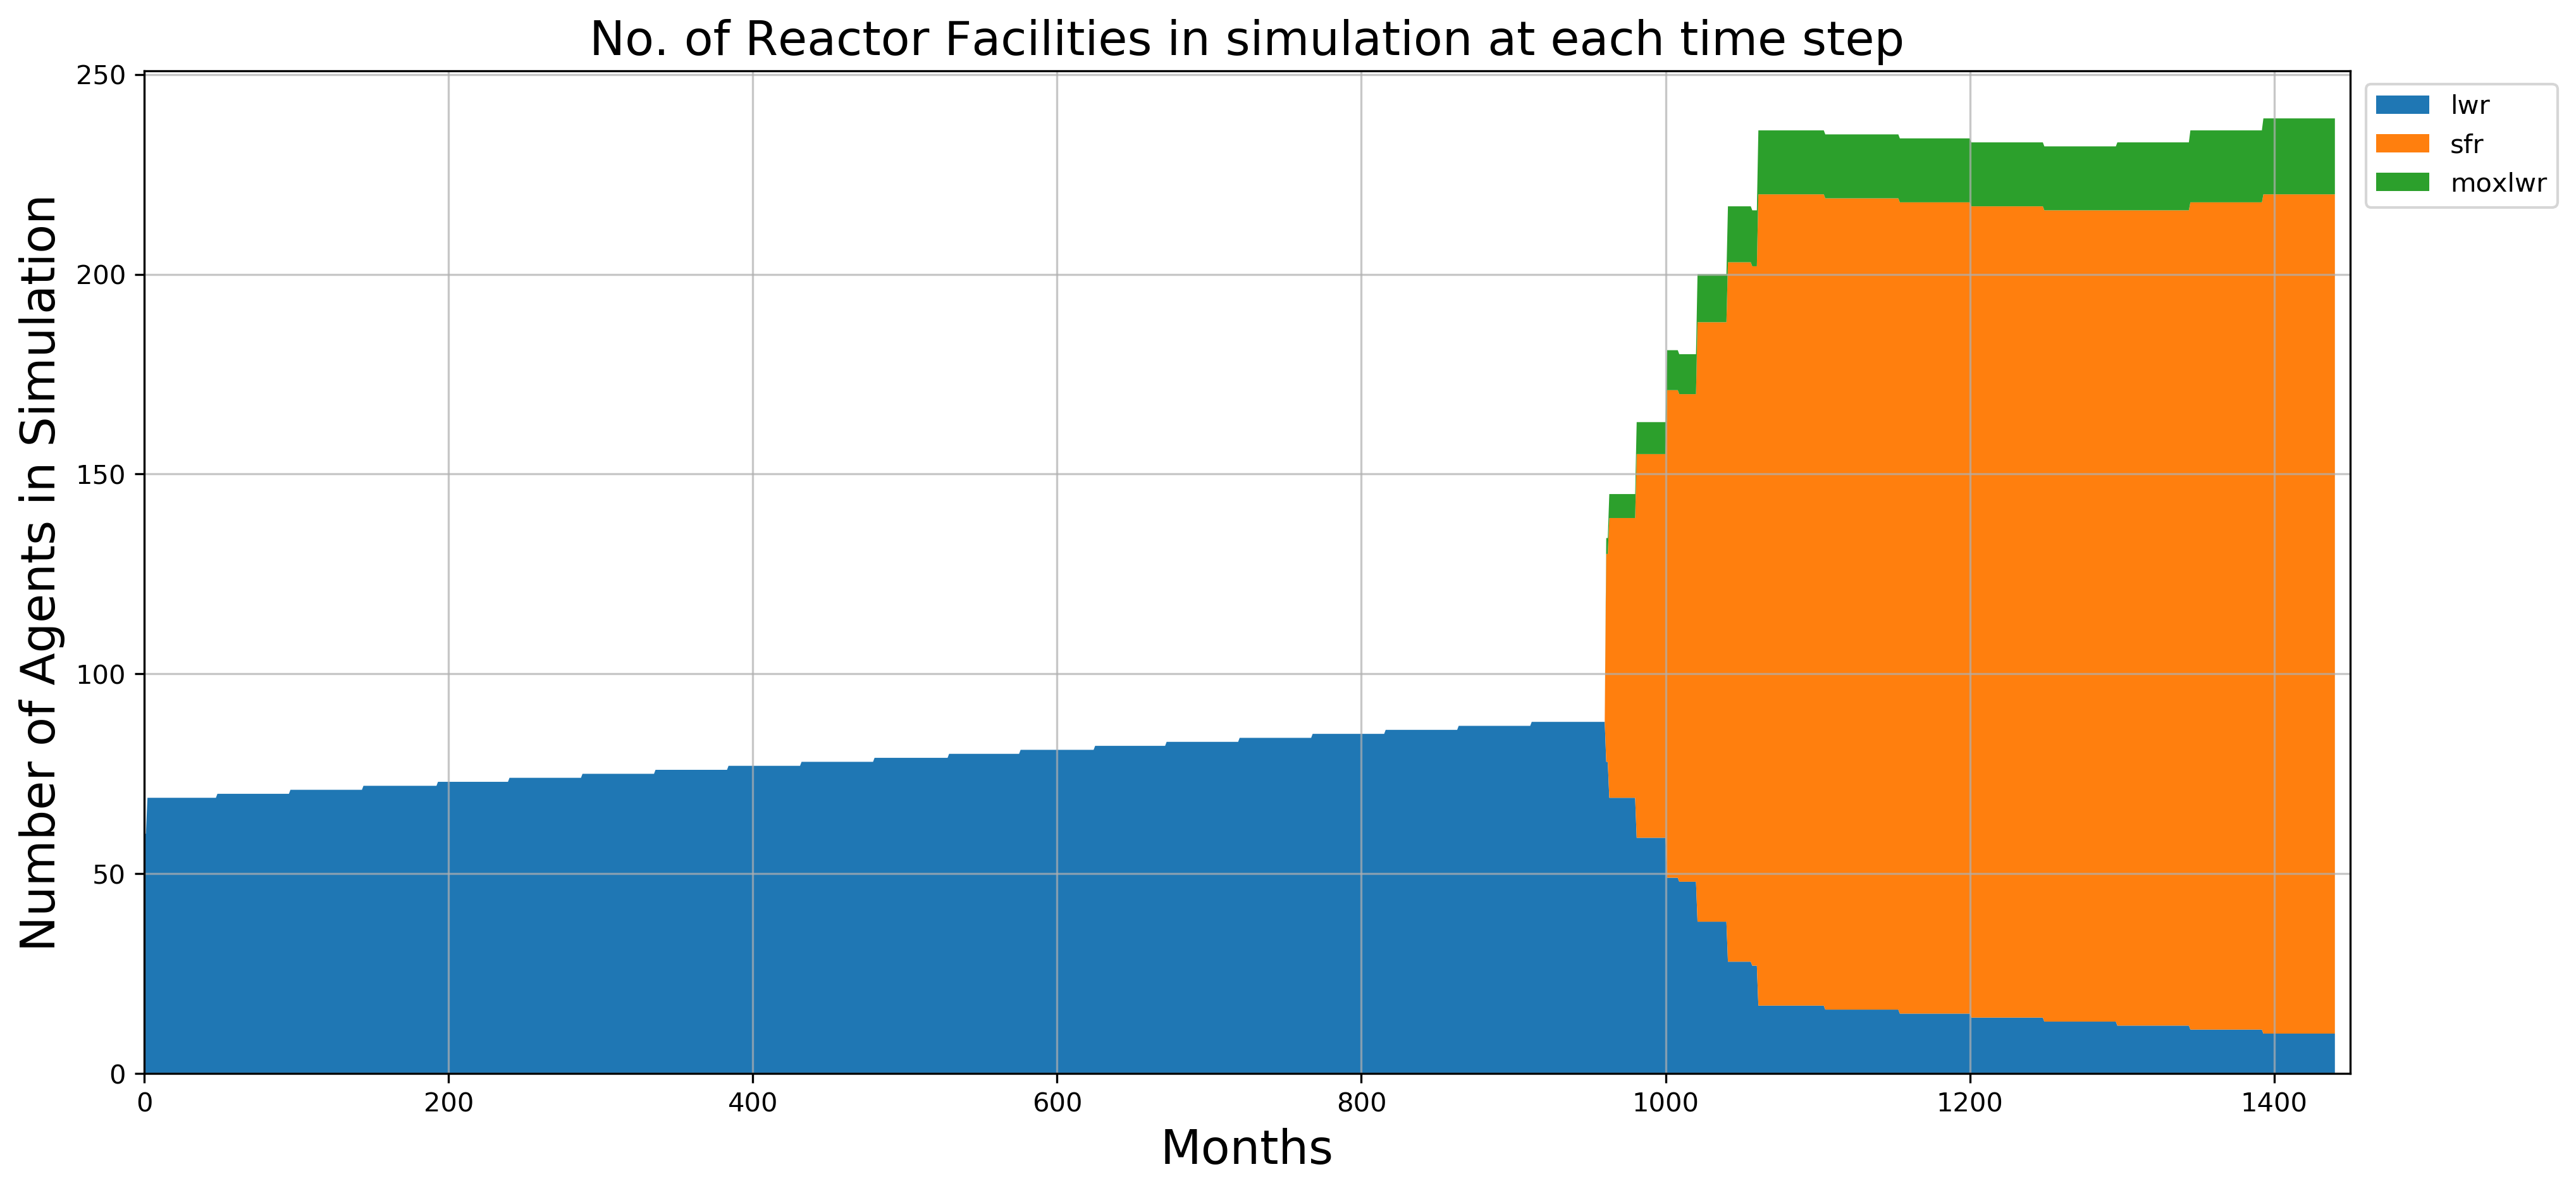
\includegraphics[width=\textwidth]{images/eg30-stack_reactor.png}
\end{center}
\caption{Time dependent deployment of reactor facilities in 
the EG01-30 linearly increasing power demand transition scenario. 
\deploy automatically deploys reactor facilities 
to set up a supply chain to meet constant power demand of $60000+250t/12$ MW
during a transition from \glspl{LWR} to \glspl{SFR}}.
\end{figure}
\end{frame}

\begin{frame}
\frametitle{Best Performing Transition Scenarios}
\textbf{EG01-30: Linearly Increasing Power Demand}
\begin{figure}[htbp!]
\begin{center}
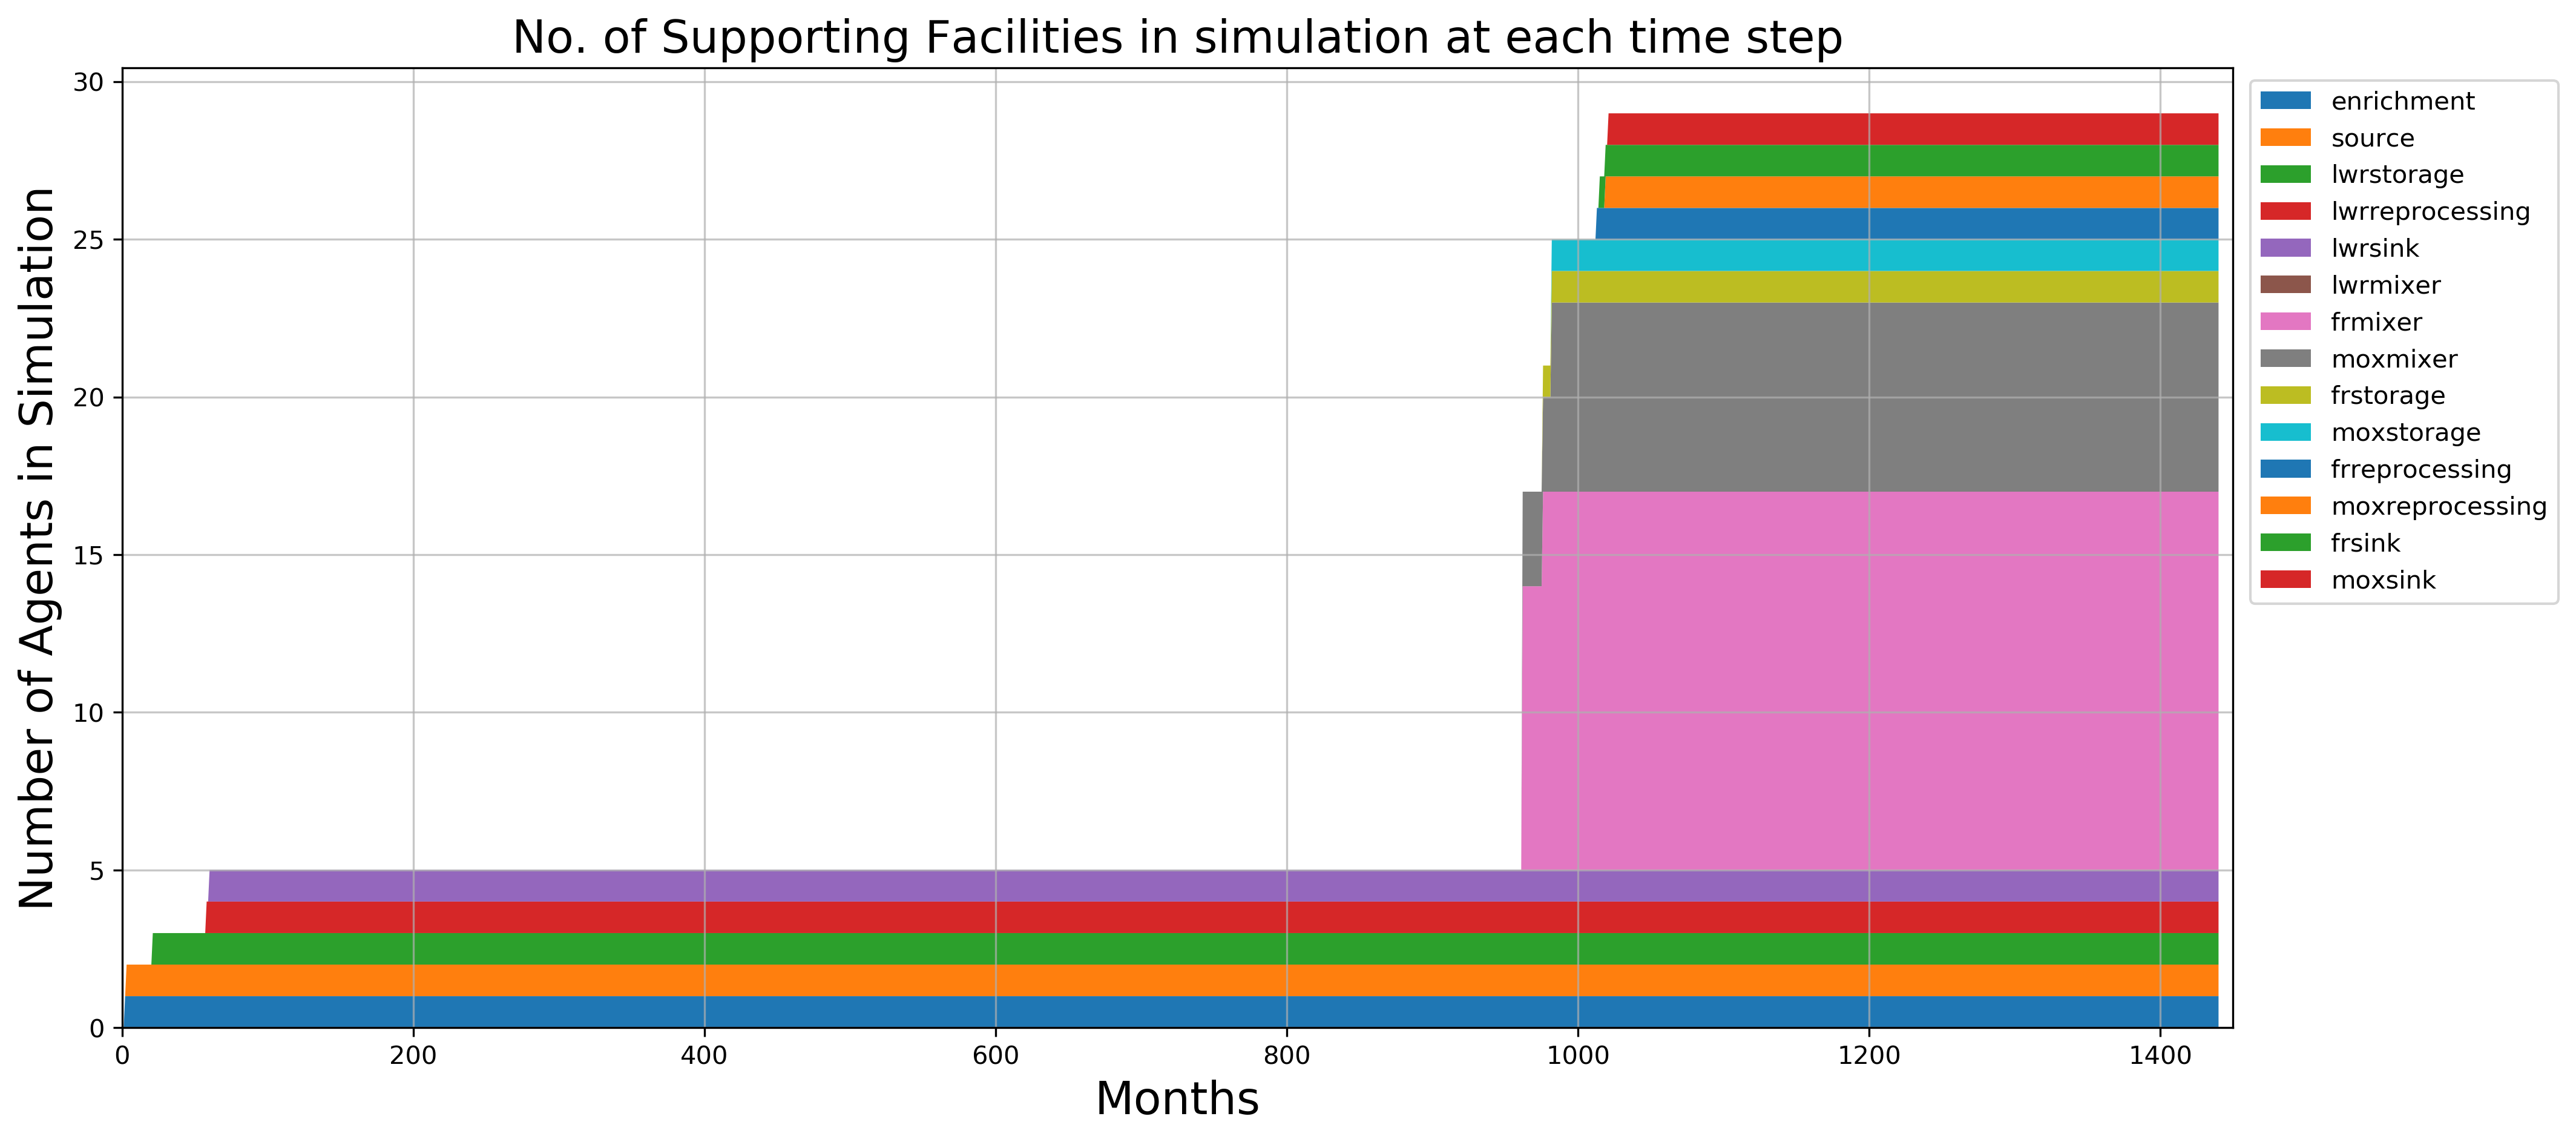
\includegraphics[width=\textwidth]{images/eg30-stack_support.png}
\end{center}
\caption{Time dependent deployment of supporting facilities in 
the EG01-30 linearly increasing power demand transition scenario. 
\deploy automatically deploys reactor facilities 
to set up a supply chain to meet constant power demand of $60000+250t/12$ MW
during a transition from \glspl{LWR} to \glspl{SFR}}.
\end{figure}
\end{frame}

\begin{frame}
\frametitle{Best Performing Transition Scenarios}
\textbf{Undersupply and under capacity of commodities for the best performing transition scenarios} 
\begin{table}[]
\centering
\caption{Undersupply/capacity of commodities for the best performing EG01-EG23,24,29,30 transition scenarios.}
\label{tab:all-power}
\footnotesize
\begin{tabularx}{\textwidth}{l|RRRR}
\hline
& \multicolumn{3}{|c}{\textbf{Undersupplied Time Steps}} \\ \hline
\textbf{Transition Scenario} & EG01-EG23 & 
EG01-EG24 & EG01-EG29 & 
EG01-EG30 \\ 
\textbf{Power Demand} &Constant&Linearly Increasing&Constant&Linearly Increasing \\
\textbf{Prediction Method} &\texttt{poly}&\texttt{fft}&\texttt{poly}& \texttt{fft}\\
\textbf{Power Supply Buffer [MW]} &0&6000&0&8000 \\ \hline
\textbf{Commodities} \\ 
Natural Uranium		    & 2 	& 3  &  1  & 1 \\ 
\gls{LWR} Fuel     	    & 4 	& 6  &  1  & 2\\ 
\gls{SFR} Fuel     	    &  0 	& 0  &  2  & 2\\ 
\gls{MOX} \gls{LWR} Fuel &-&-&2&2 \\
Power      				&  6 	& 7  &  4 &  5\\ 
\gls{LWR} Spent Fuel	& 1 	& 1  & 1 & 1\\ 
\gls{SFR} Spent Fuel     	    &  1 	& 1  &  1  & 1\\ 
\gls{MOX} \gls{LWR} Spent Fuel &-&-&1&1 \\ \hline 
\end{tabularx}
\end{table}

\end{frame}

\begin{frame}
\frametitle{Conclusion}
These results demonstrate that by carefully selecting \deploy 
parameters, we are able to \textbf{effectively automate deployment}
of reactor and supporting facilities to set up 
constant and linearly increasing power demand transition scenarios
for EG01-23, EG01-24, EG01-29, and EG01-30 with minimal 
power undersupply. 
\vspace{1em}
\\
Not completely eliminating undersupply and under capacity of 
commodities in the simulation is expected 
since without time series data 
at the beginning of the simulation, \deploy takes a few 
time steps to collect time series data about power demand 
to predict and start deploying reactor and supporting 
fuel cycle facilities. 

\end{frame}